\chapter{RESULTS}
\label{chap-four}
	In this chapter we first discuss the performance of the Intra - Subject classification. Later we discuss the performance of Inter - subject Classification.
    
    \section{Measuring Performance}
    
    Apart from the classification accuracy the two measures of performances used are ``True positive rate'' and ``False Positive rate''. Say if we must have to identify the class $c_i$ among $c_1, c_2 \dots c_n$, the true positive rate measures the percentage of patterns classified correctly as class $c_1$, whereas the false positive rate measures the percentage of patterns which do not belong to class $c_1$ but are classified as class $c_1$.
    
    True Positive rate (TPR) is computed as given by Equation \ref{EQ:chap4TPR}.
    
    \begin{equation}
    	TPR = \frac{TP}{TP + FN} \;,
    	\label{EQ:chap4TPR}
    \end{equation}
    
    \noindent where TP is the number of true positive samples and FN is the number of false negative samples. The confusion matrix shown in Table \ref{Table:chap4ConfusinMatrix} gives better understanding of true positives(TP), false positives(FP), true negatives(TN) and false negatives(FN).
    
\begin{table}[]
\centering
\caption{Confusion Matrix}
\label{Table:chap4ConfusinMatrix}
\begin{tabular}{cc|c|c|}
\cline{3-4}
                                                                           &  & \multicolumn{2}{c|}{Predicted Condition}                                                                                      \\ \cline{2-4} 
\multicolumn{1}{c|}{}                                                                            & Total Classification & Predicted Positive                                            & Predicted Negative                                            \\ \hline
\multicolumn{1}{|c|}{\multirow{2}{*}{\begin{tabular}[c]{@{}c@{}}True \\ Condition\end{tabular}}} & Actually Positive    & \begin{tabular}[c]{@{}c@{}}True Positive\\ (TP)\end{tabular}  & \begin{tabular}[c]{@{}c@{}}False Negative\\ (FN)\end{tabular} \\ \cline{2-4} 
\multicolumn{1}{|c|}{}                                                                           & Actually Negative    & \begin{tabular}[c]{@{}c@{}}False Positive\\ (FP)\end{tabular} & \begin{tabular}[c]{@{}c@{}}True Negative\\ (TN)\end{tabular}  \\ \hline
\end{tabular}
\end{table}

	Similar to TPR, false positive rates (FPR) can be calculated using Equation \ref{EQ:chap4FPR}.
    
    \begin{equation}
    	FPR = \frac{FP}{FP + TN} \;,
    	\label{EQ:chap4FPR}
    \end{equation}
        \section{Similarity in EEG signals}
        Figure \ref{fig:chap41}, Figure \ref{fig:chap43} and Figure \ref{fig:chap45} show the mean of amplitude of the feature vectors for calculation, breathing and singing tasks. Figure \ref{fig:chap42}, Figure \ref{fig:chap44} and Figure \ref{fig:chap46} show the variance of amplitude of the feature vectors. The description of these tasks is given by Table \ref{Tasks}. As we can see, from the ``mean'' graphs, EEG bands for four different test subjects follow similar patterns for the same task performed, although they vary slightly. As a result, classifying EEG signals is difficult. Also, note that the variance for Subject 1 is very low. This maybe because the brain wave signatures of Subject 1 for different tasks are closer compared to other subjects. 
        
	\begin{figure}[hbtp]
    	\centering
    	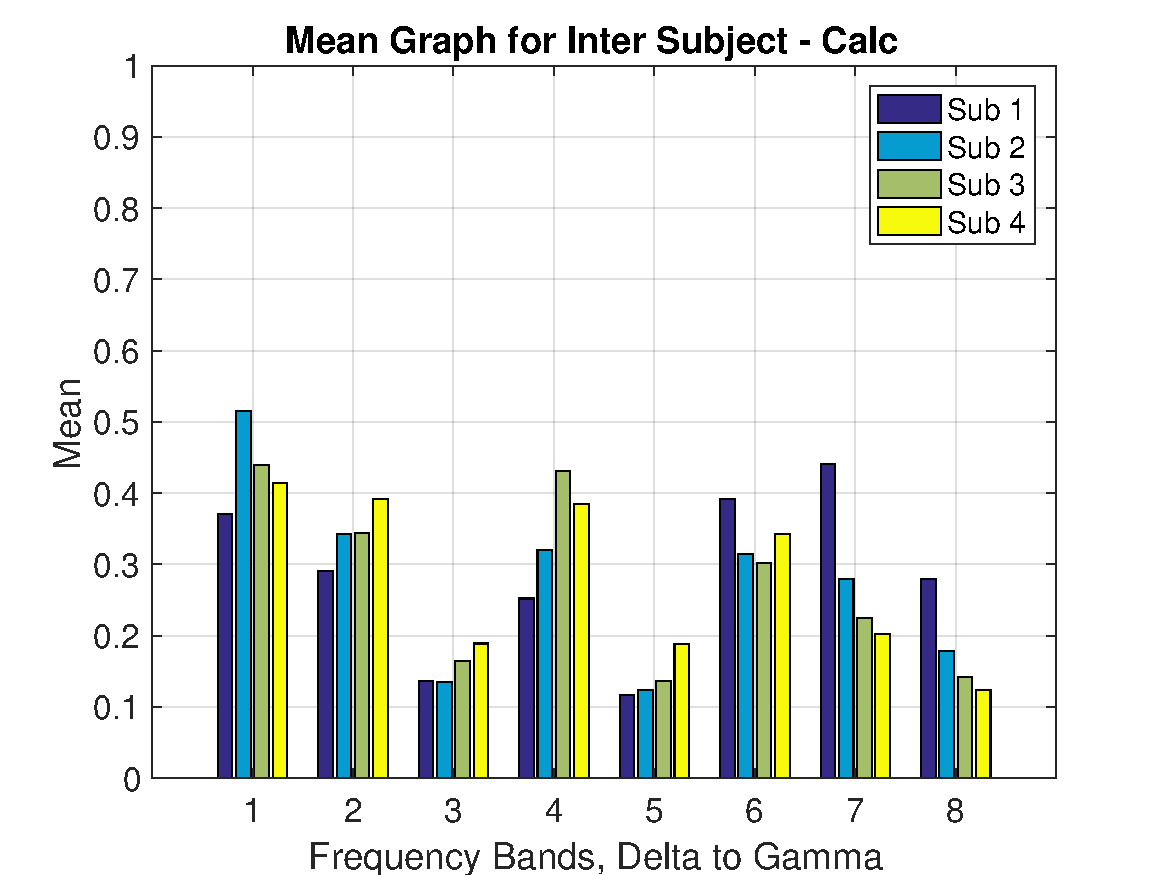
\includegraphics[width=0.9\textwidth]{Chapter-4/1}
    	\caption{Mean of each EEG band for Calculation task}
    	\label{fig:chap41}
    \end{figure}

    \begin{figure}[hbtp]
    	\centering
    	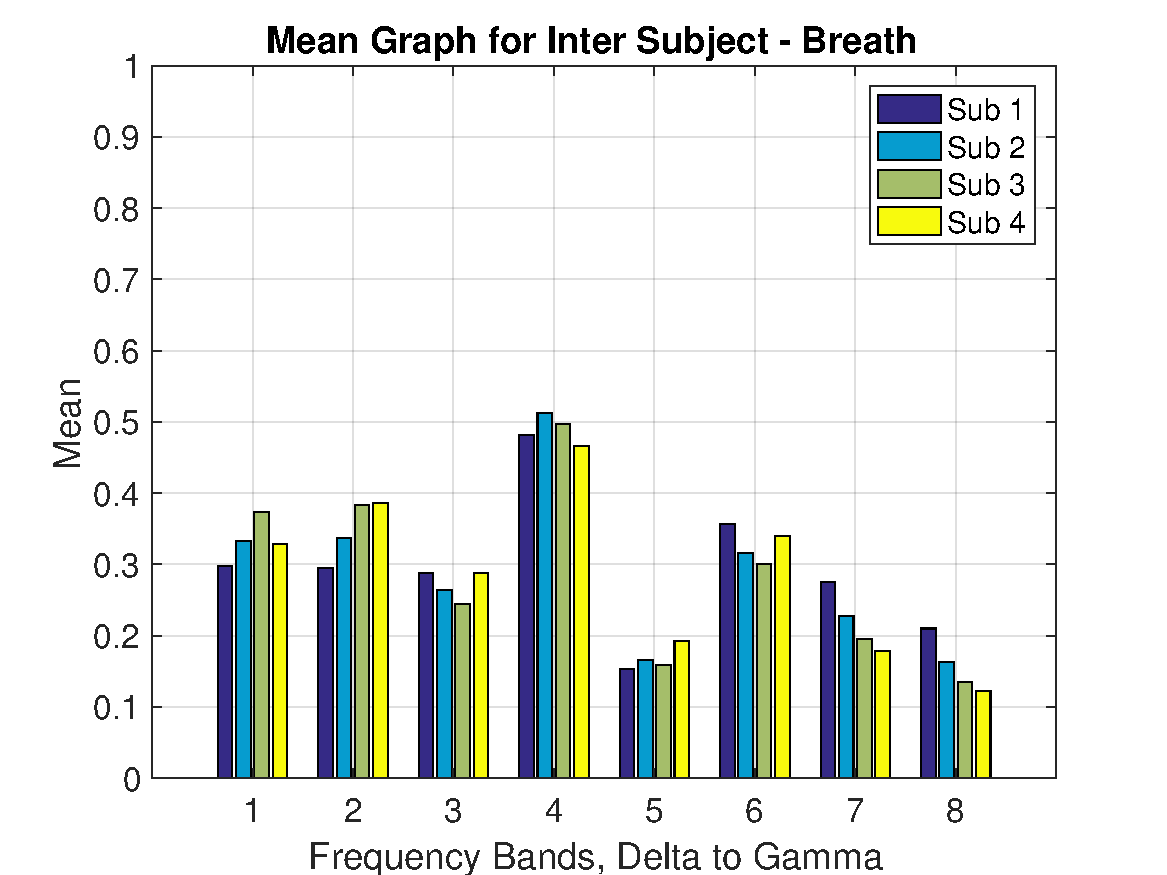
\includegraphics[width=0.9\textwidth]{Chapter-4/3}
    	\caption{Mean of each EEG band for Breathing task}
    	\label{fig:chap43}
    \end{figure}

    \begin{figure}[hbtp]
    	\centering
    	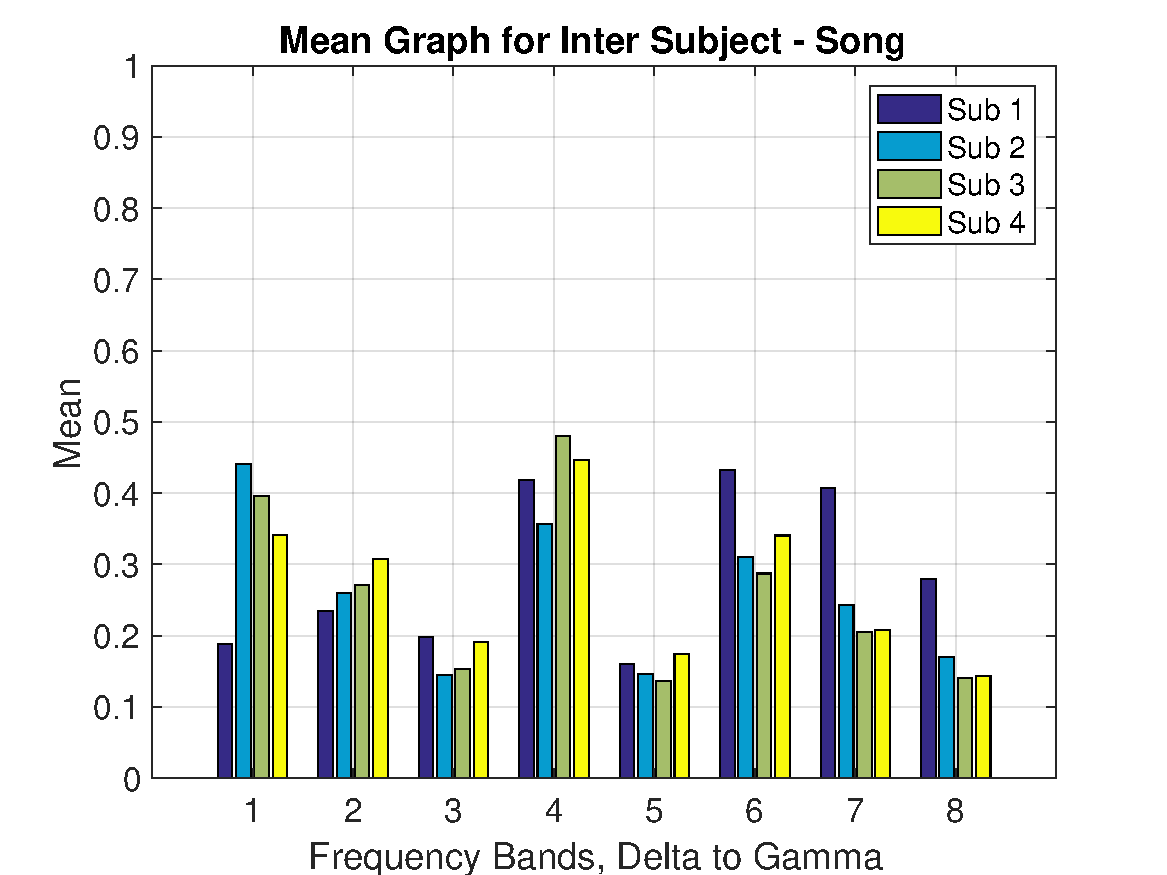
\includegraphics[width=0.9\textwidth]{Chapter-4/5}
    	\caption{Mean of each EEG band for Singing task}
    	\label{fig:chap45}
    \end{figure}

    \begin{figure}[hbtp]
    	\centering
    	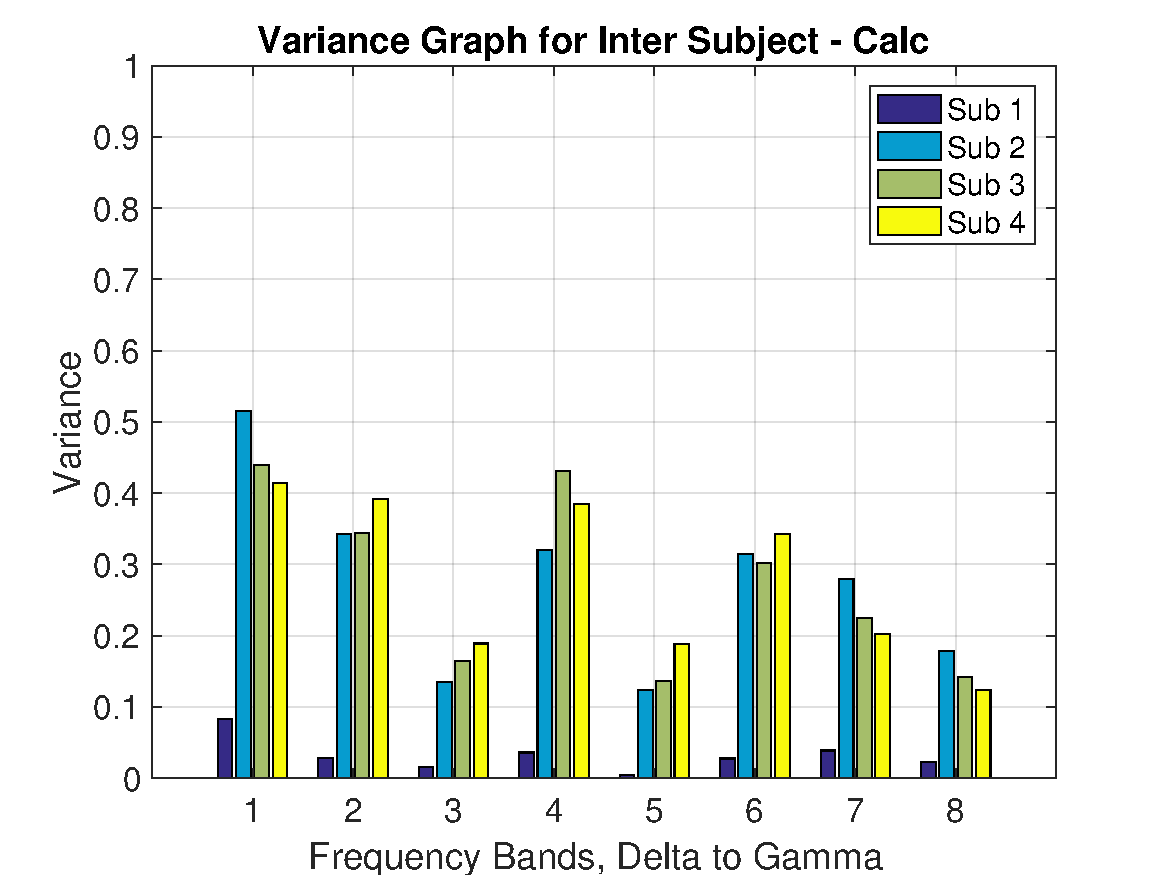
\includegraphics[width=0.9\textwidth]{Chapter-4/2}
    	\caption{Variance of each EEG band for Calculation task}
    	\label{fig:chap42}
    \end{figure}

    \begin{figure}[hbtp]
    	\centering
    	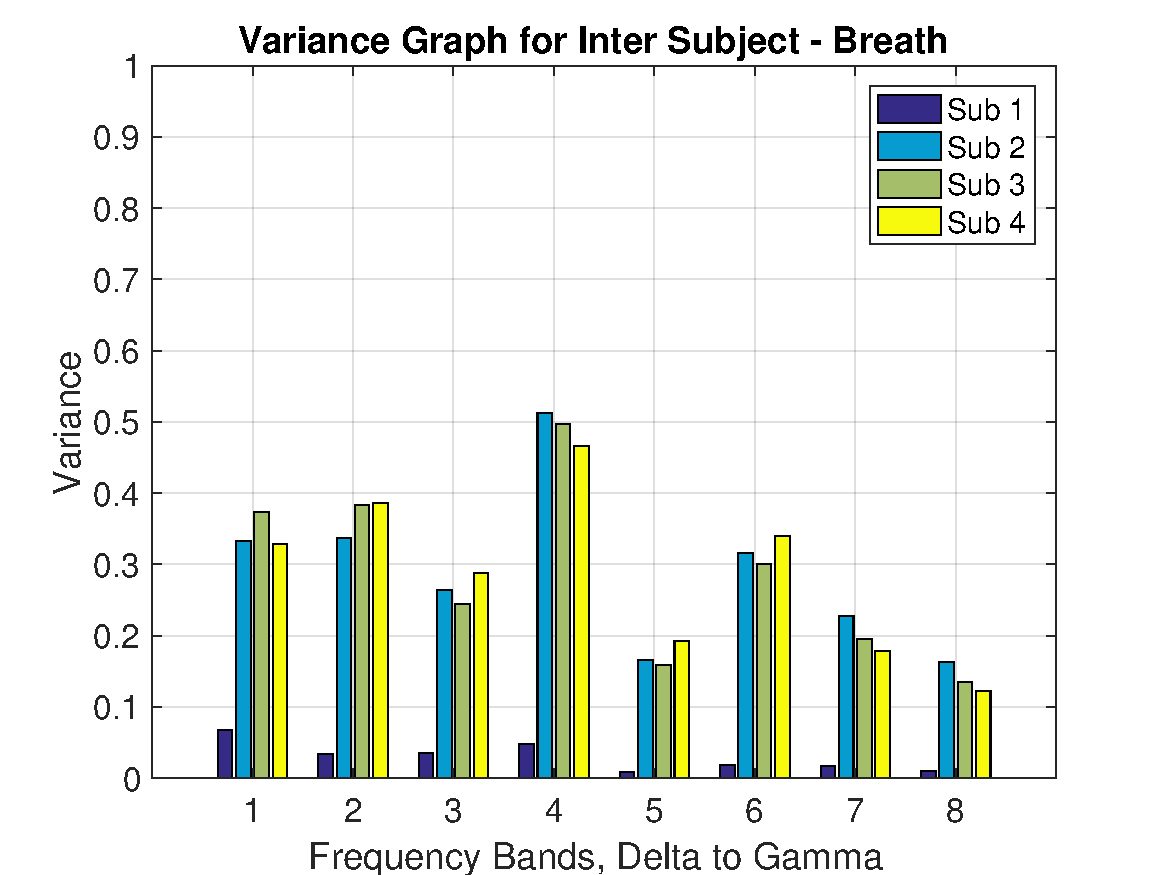
\includegraphics[width=0.9\textwidth]{Chapter-4/4}
    	\caption{Variance of each EEG band for Breathing task}
    	\label{fig:chap44}
    \end{figure}

    \begin{figure}[hbtp]
    	\centering
    	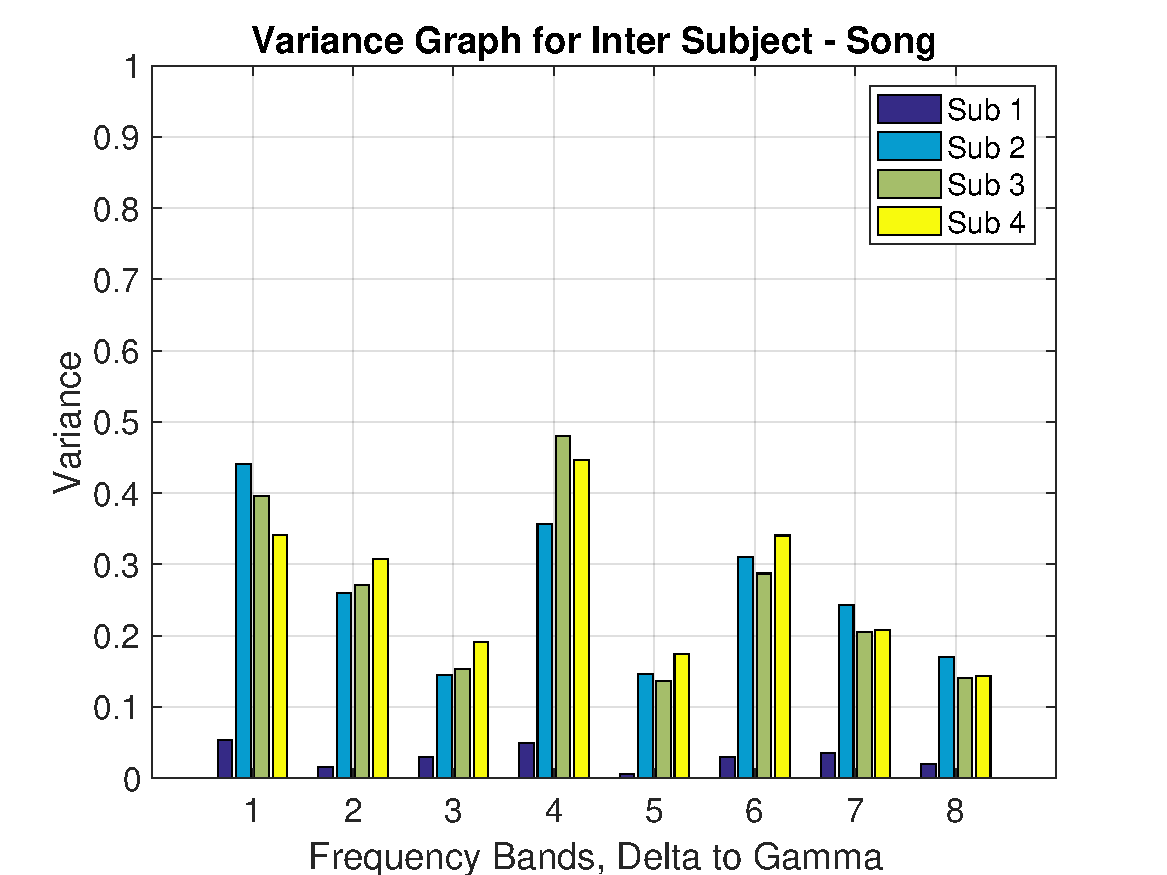
\includegraphics[width=0.9\textwidth]{Chapter-4/6}
    	\caption{Variance of each EEG band for Singing task}
    	\label{fig:chap46}
    \end{figure}

    \FloatBarrier

    \section{Classifier Performance}
    Performance of the Mahalanobis Distance classifier, the Neural Network classifier and the SVM classifier are discussed in this section. As discussed in Section \ref{Chap3:Classifiers}, we consider two types of EEG data classification. First is to identify the ``task'' performed by the subject. We call this ``Intra-subject classification''. Second type of classification is to identify the subject among group of subject performing similar tasks. We call this ``Inter-subject classification''. Here task refers to the brain activity like doing mathematical calculation, concentrating on breathing or mentally singing a song(refer Table \ref{Tasks} for more details).
    
    We also need to consider comparison of baseline performance verses classifier performance. For example, if the feature vectors of all the classes are uniformly distributed, then, if we randomly choose a class among given classes, the probability of being right is given by Equation \ref{EQ:chap4base}.

    	\begin{equation}
    		P =  \frac{1}{N} \;,
    		\label{EQ:chap4base}
    	\end{equation}

    	\noindent where N is the total number of classes. We call this the ``baseline performance''.

    \subsection{Intra-subject Classification}
    For this experiment, we collected data from four different test subjects performing three different tasks repeated five times each. As discussed in Section \ref{Chap3:Classifiers}, training and testing split was 70\% and 30\% respectively.
    
    \subsubsection{Mahalanobis Distance}
    Table \ref{MICT} and Figure \ref{fig:chap4IntraMT} show the overall accuracy of the Mahalanobis distance classifier for intra-subject classification. Table \ref{MICTPR} and Figure \ref{fig:chap4IntraMTPR} show the TPR for different tasks using the Mahalanobis distance classifier. Also, Table \ref{MICFPR} and Figure \ref{fig:chap4IntraMFPR} show the FPR for different tasks using the Mahalanobis distance classifier.
		\begin{table}[h!]
			\centering
			\caption{Intra-subject Classification using Mahalanobis Distance, Total Accuracy}
			\label{MICT}
			\begin{tabular}{c c c c}
				\hline
				Sub &Min &Max &Average\\\hline
				1 &33.33 &55.56 &44.89\\
				2 &44.44 &66.67 &55.78\\
				3 &35.56 &46.67 &42.67\\
				4 &44.44 &71.11 &61.56\\
			\end{tabular}
		\end{table}
        
        \begin{figure}[hbtp]
	    	\centering
	    	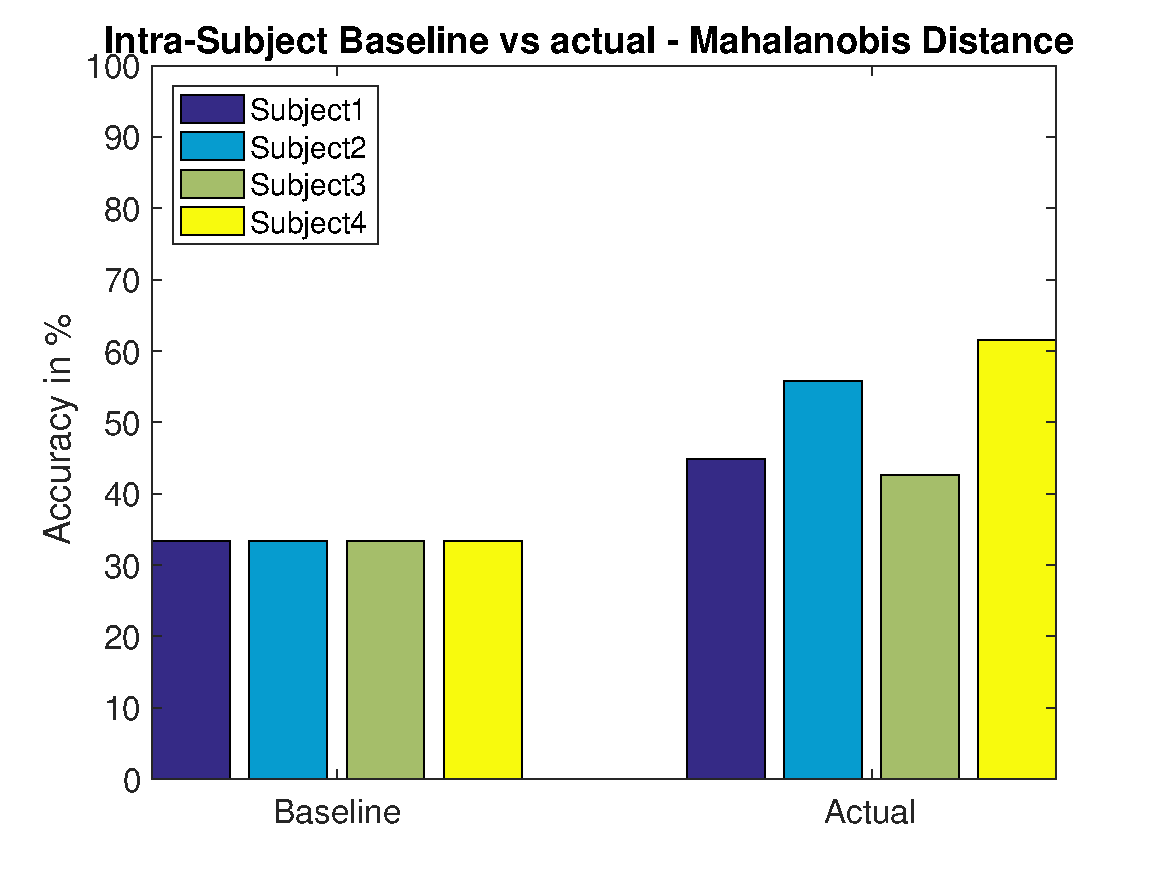
\includegraphics[width=0.90\textwidth]{Chapter-4/base_tm}
	    	\caption{Total accuracy for Intra-subject classification using the Mahalanobis Distance Classifier}
	    	\label{fig:chap4IntraMT}
    	\end{figure}

    	\begin{figure}[hbtp]
	    	\centering
	    	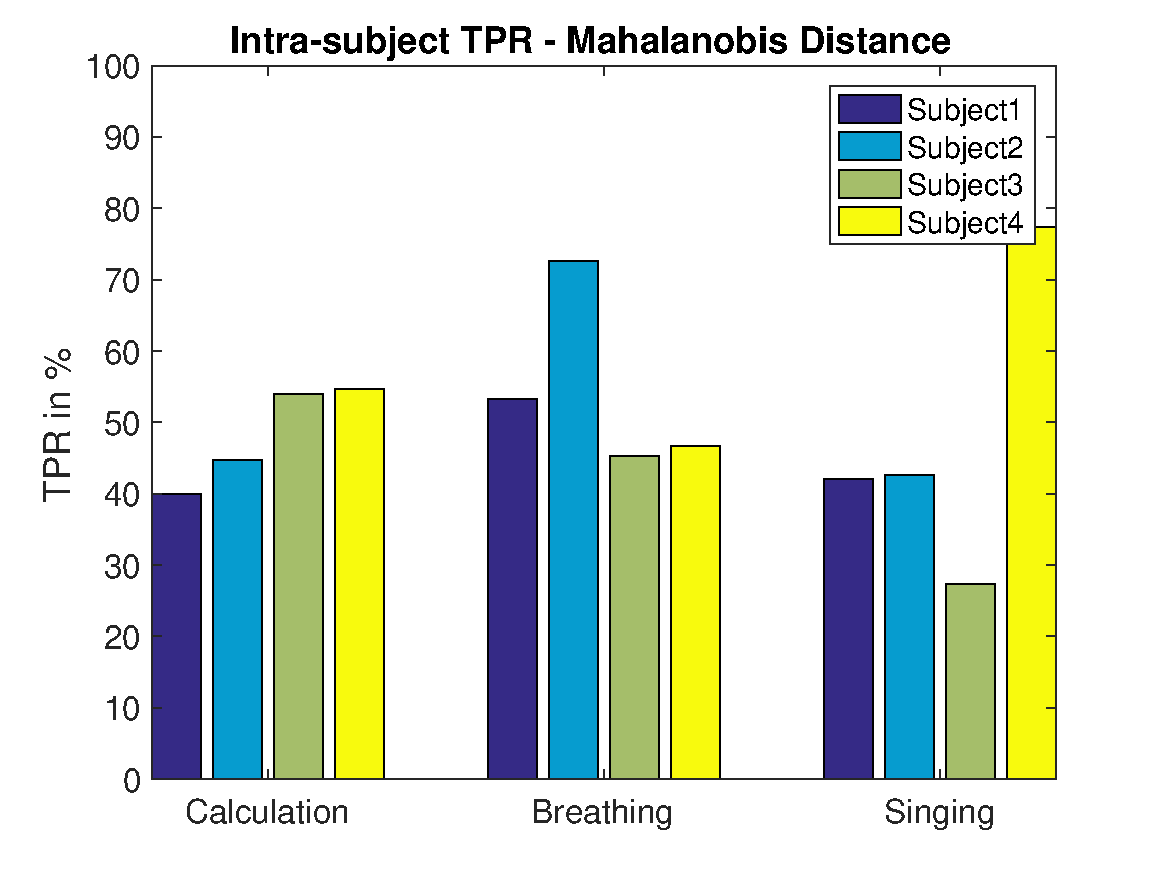
\includegraphics[width=0.90\textwidth]{Chapter-4/base_tprm}
	    	\caption{TPR for Intra-subject classification using the Mahalanobis Distance Classifier}
	    	\label{fig:chap4IntraMTPR}
    	\end{figure}

    	\begin{figure}[hbtp]
	    	\centering
	    	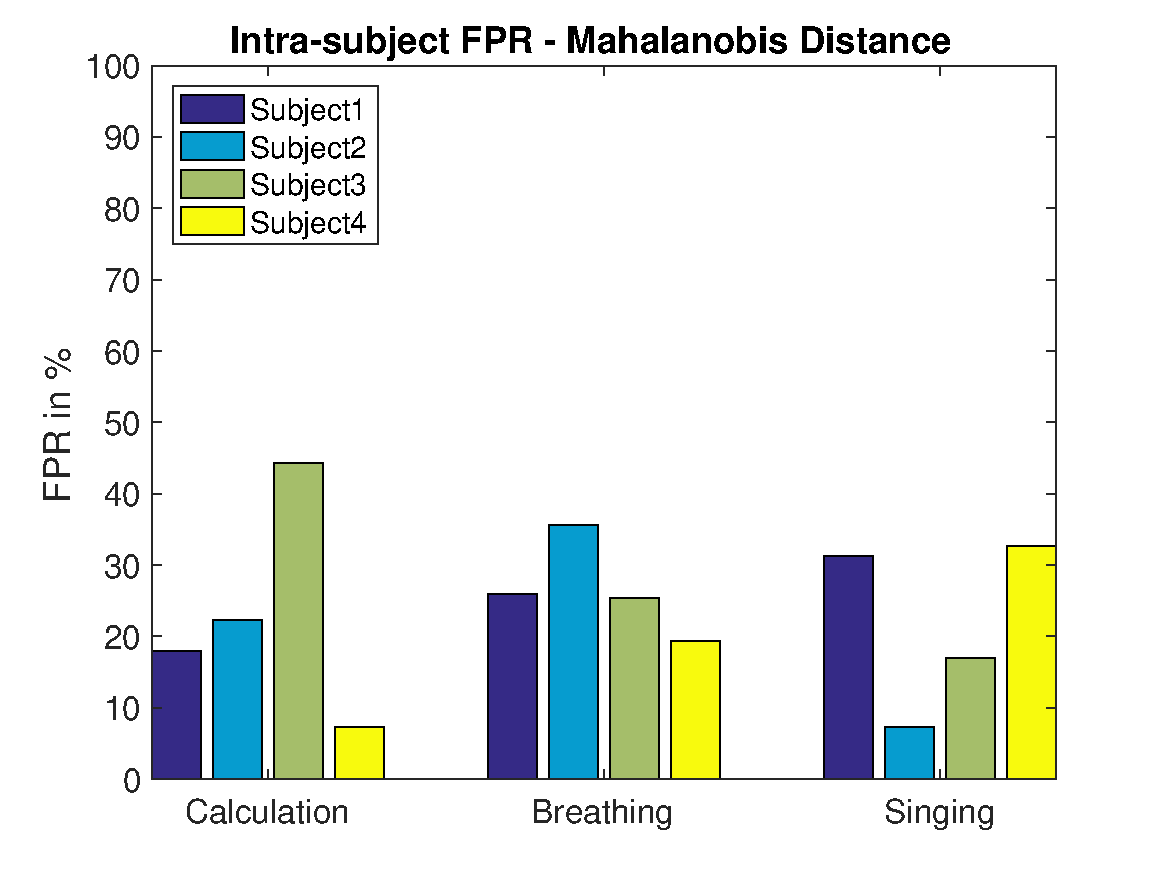
\includegraphics[width=0.90\textwidth]{Chapter-4/base_fprm}
	    	\caption{FPR for Intra-subject classification using the Mahalanobis Distance Classifier}
	    	\label{fig:chap4IntraMFPR}
    	\end{figure}

		\begin{table}[h!]
			\centering
			\caption{Intra-subject Classification using Mahalanobis Distance, TPR for Calculation, Breathing and Singing Task}
			\label{MICTPR}
			\subfloat[Calculation]{
			\begin{tabular}{c c c c}
				\hline
				Sub &Min &Max &Average\\\hline
				1 &20.00 &66.67 &40.00\\
				2 &26.67 &73.33 &44.67\\
				3 &20.00 &80.00 &54.00\\
				4 &33.33 &73.33 &54.67\\
			\end{tabular}
			}\hfill
			\subfloat[Breathing]{
			\begin{tabular}{c c c c}
				\hline
				Sub &Min &Max &Average\\\hline
				1 &40.00 &73.33 &53.33\\
				2 &60.00 &86.67 &72.67\\
				3 &26.67 &73.33 &45.33\\
				4 &20.00 &73.33 &46.67\\
			\end{tabular}
			}\\
			\subfloat[Singing]{
			\begin{tabular}{c c c c}
				\hline
				Sub &Min &Max &Average\\\hline
				1 &13.33 &66.67 &42.00\\
				2 &26.67 &73.33 &42.67\\
				3 &13.33 &66.67 &27.33\\
				4 &60.00 &93.33 &77.33\\
			\end{tabular}
			}
		\end{table}	

		\begin{table}[h!]
			\centering
			\caption{Intra-subject Classification using Mahalanobis Distance, FPR for Calculation, Breathing and Singing Task}
			\label{MICFPR}
			\subfloat[Calculation]{
			\begin{tabular}{c c c c}
				\hline
				Sub &Min &Max &Average\\\hline
				1 &3.33 &36.67  &18.00\\
				2 &13.33 &40.00 &22.33\\
				3 &33.33 &60.00 &44.33\\
				4 &0.00 &16.67  &7.33\\
			\end{tabular}
			}\hfill
			\subfloat[Breathing]{
			\begin{tabular}{c c c c}
				\hline
				Sub &Min &Max &Average\\\hline
				1 &20.00 &36.67 &26.00\\
				2 &23.33 &53.33 &35.67\\
				3 &6.67 &43.33  &25.33\\
				4 &3.33 &36.67  &19.33\\
			\end{tabular}
			}\\
			\subfloat[Singing]{
			\begin{tabular}{c c c c}
				\hline
				Sub &Min &Max &Average\\\hline
				1 &10.00 &46.67 &31.33\\
				2 &0.00 &13.33  &7.33\\
				3 &6.67 &23.33  &17.00\\
				4 &20.00 &53.33 &32.67\\
			\end{tabular}
			}
		\end{table}

        \FloatBarrier
    \subsubsection{Neural Networks}
    Table \ref{NICT} and Figure \ref{fig:chap4IntraNT} show the overall accuracy of the Neural Networks classifier for intra-subject classification. Table \ref{NICTPR} and Figure \ref{fig:chap4IntraNTPR} show the TPR for different tasks using the Neural Networks classifier. Also, Table \ref{NICFPR} and Figure \ref{fig:chap4IntraNFPR} show the FPR for different tasks using the Neural Networks classifier.
    
		\begin{table}[h!]
			\centering
			\caption{Intra-subject Classification using Neural Networks, Total Accuracy}
			\label{NICT}
			\begin{tabular}{c c c c}
				\hline
				Sub &Min &Max &Average\\\hline
				1 &53.33 &64.44 &58.22\\
				2 &57.78 &73.33 &65.11\\
				3 &44.44 &55.56 &48.44\\
				4 &62.22 &73.00 &66.67\\
			\end{tabular}
		\end{table}
        
        \begin{figure}[hbtp]
	    	\centering
	    	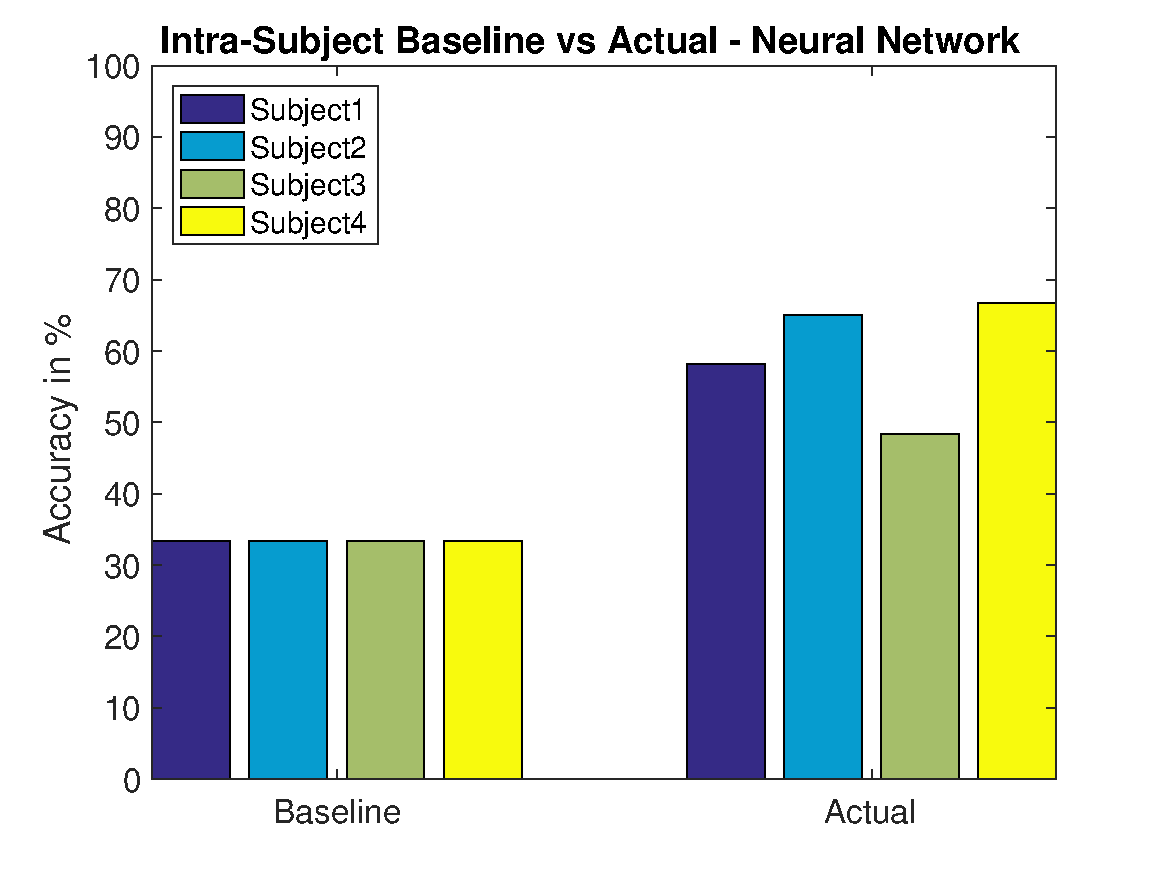
\includegraphics[width=0.90\textwidth]{Chapter-4/base_tn}
	    	\caption{Total accuracy for Intra-subject classification using the Neural Network Classifier}
	    	\label{fig:chap4IntraNT}
    	\end{figure}

    	\begin{figure}[hbtp]
	    	\centering
	    	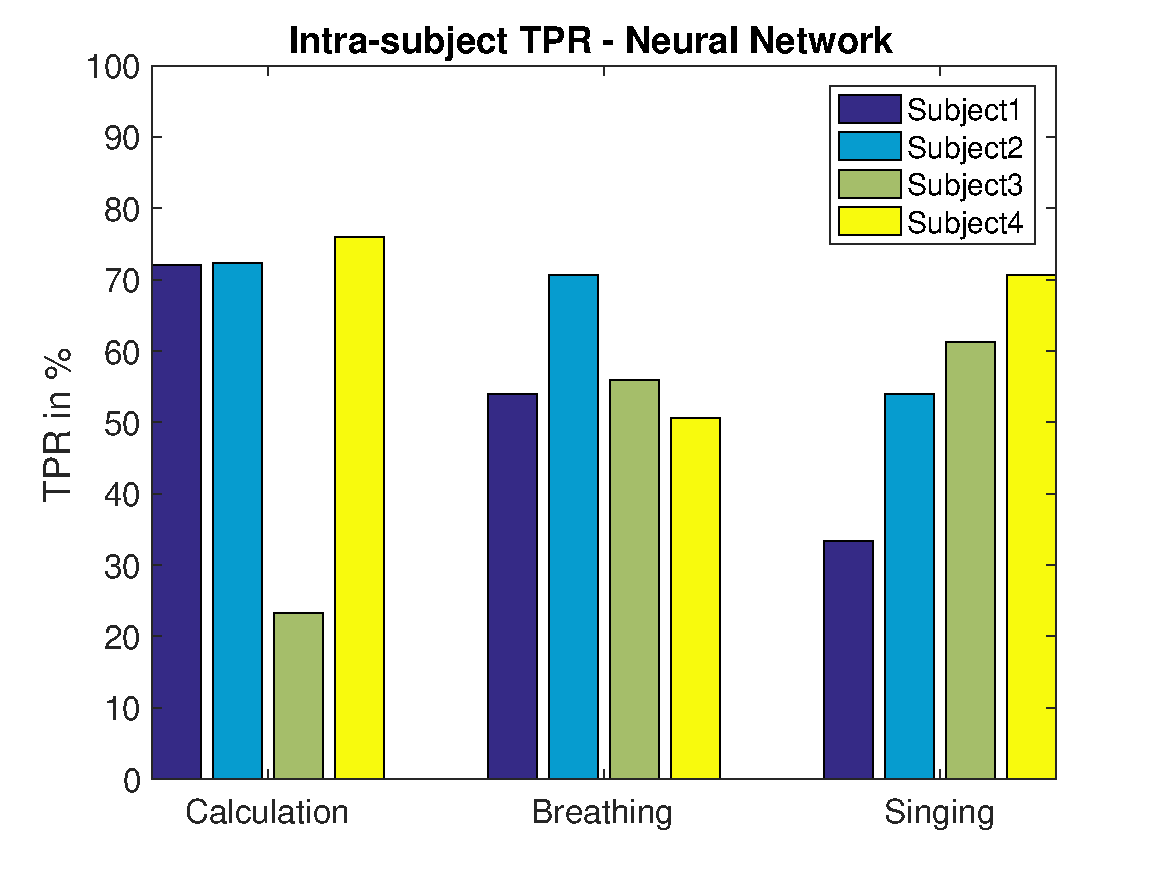
\includegraphics[width=0.90\textwidth]{Chapter-4/base_tprn}
	    	\caption{TPR for Intra-subject classification using the Neural Network Classifier}
	    	\label{fig:chap4IntraNTPR}
    	\end{figure}

    	\begin{figure}[hbtp]
	    	\centering
	    	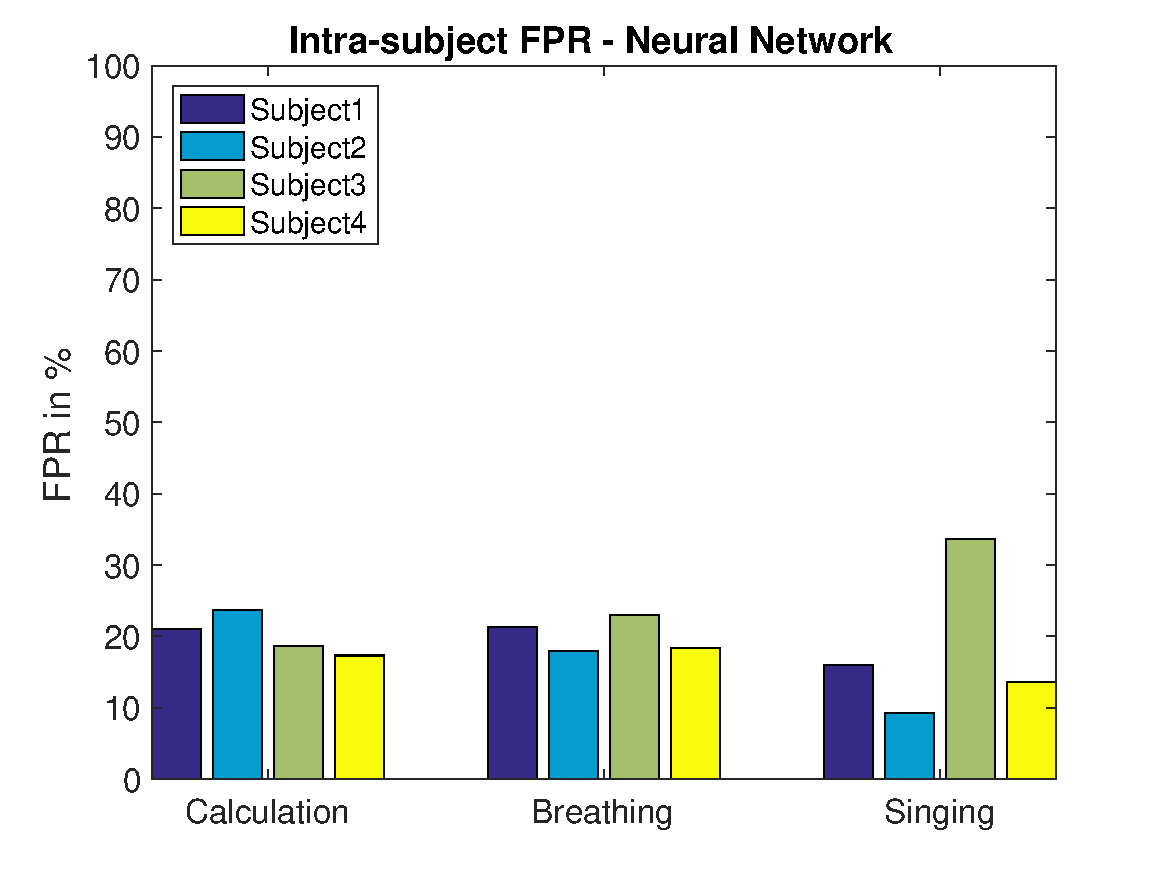
\includegraphics[width=0.90\textwidth]{Chapter-4/base_fprn}
	    	\caption{FPR for Intra-subject classification using the Neural Network Classifier}
	    	\label{fig:chap4IntraNFPR}
    	\end{figure}


		\begin{table}[h!]
			\centering
			\caption{Intra-subject Classification using Neural Networks, TPR for Calculation, Breathing and Singing Task}
			\label{NICTPR}
			\subfloat[Calculation]{
			\begin{tabular}{c c c c}
				\hline
				Sub &Min &Max &Average\\\hline
				1 &60.00 &86.67 &72.00\\
				2 &46.67 &93.33 &72.33\\
				3 &6.67 &33.33  &23.33\\
				4 &66.67 &93.33 &76.00\\
			\end{tabular}
			}\hfill
			\subfloat[Breathing]{
			\begin{tabular}{c c c c}
				\hline
				Sub &Min &Max &Average\\\hline
				1 &33.33 &66.67 &54.00\\
				2 &66.67 &86.67 &70.67\\
				3 &26.67 &66.67 &56.00\\
				4 &33.33 &66.67 &50.67\\
			\end{tabular}
			}\\
			\subfloat[Singing]{
			\begin{tabular}{c c c c}
				\hline
				Sub &Min &Max &Average\\\hline
				1 &13.33 &53.33 &33.33\\
				2 &26.67 &80.00 &54.00\\
				3 &40.00 &86.67 &61.33\\
				4 &60.00 &93.33 &70.67\\
			\end{tabular}
			}
		\end{table}

		\begin{table}[h!]
			\centering
			\caption{Intra-subject Classification using Neural Networks, FPR for Calculation, Breathing and Singing Task}
			\label{NICFPR}
			\subfloat[Calculation]{
			\begin{tabular}{c c c c}
				\hline
				Sub &Min &Max &Average\\\hline
				1 &13.33 &36.67 &21.00\\
				2 &16.67 &30.00 &23.67\\
				3 &13.33 &33.33 &18.67\\
				4 &10.00 &33.33 &17.33\\
			\end{tabular}
			}\hfill
			\subfloat[Breathing]{
			\begin{tabular}{c c c c}
				\hline
				Sub &Min &Max &Average\\\hline
				1 &10.00 &33.33 &21.33\\
				2 &3.33 &26.67  &18.00\\
				3 &10.00 &36.67 &23.00\\
				4 &6.67 &26.67  &18.33\\
			\end{tabular}
			}\\
			\subfloat[Singing]{
			\begin{tabular}{c c c c}
				\hline
				Sub &Min &Max &Average\\\hline
				1 &10.00 &23.33 &16.00\\
				2 &3.33 &13.33  &9.33\\
				3 &20.00 &60.00 &33.67\\
				4 &3.33 &23.33  &13.67\\
			\end{tabular}
			}			
		\end{table}
		\FloatBarrier
    \subsubsection{Support Vector Machines}
    Table \ref{SICT} and Figure \ref{fig:chap4IntraST} show the overall accuracy of the SVM classifier for intra-subject classification. Table \ref{SICTPR} and Figure \ref{fig:chap4IntraSTPR} show the TPR for different tasks using the SVM classifier. Also, Table \ref{SICFPR} and Figure \ref{fig:chap4IntraSFPR} show the FPR for different tasks using the SVM classifier.
		\begin{table}[h!]
			\centering
			\caption{Intra-subject Classification using Support Vector Machines, Total Accuracy}
			\label{SICT}
			\begin{tabular}{c c c c}
				\hline
				Sub &Min &Max &Average\\\hline
				1 &40.00 &57.78 &50.67\\
				2 &55.56 &71.11 &66.44\\
				3 &33.33 &48.89 &41.11\\
				4 &57.78 &73.33 &65.56\\
			\end{tabular}
		\end{table}

		\begin{figure}[hbtp]
	    	\centering
	    	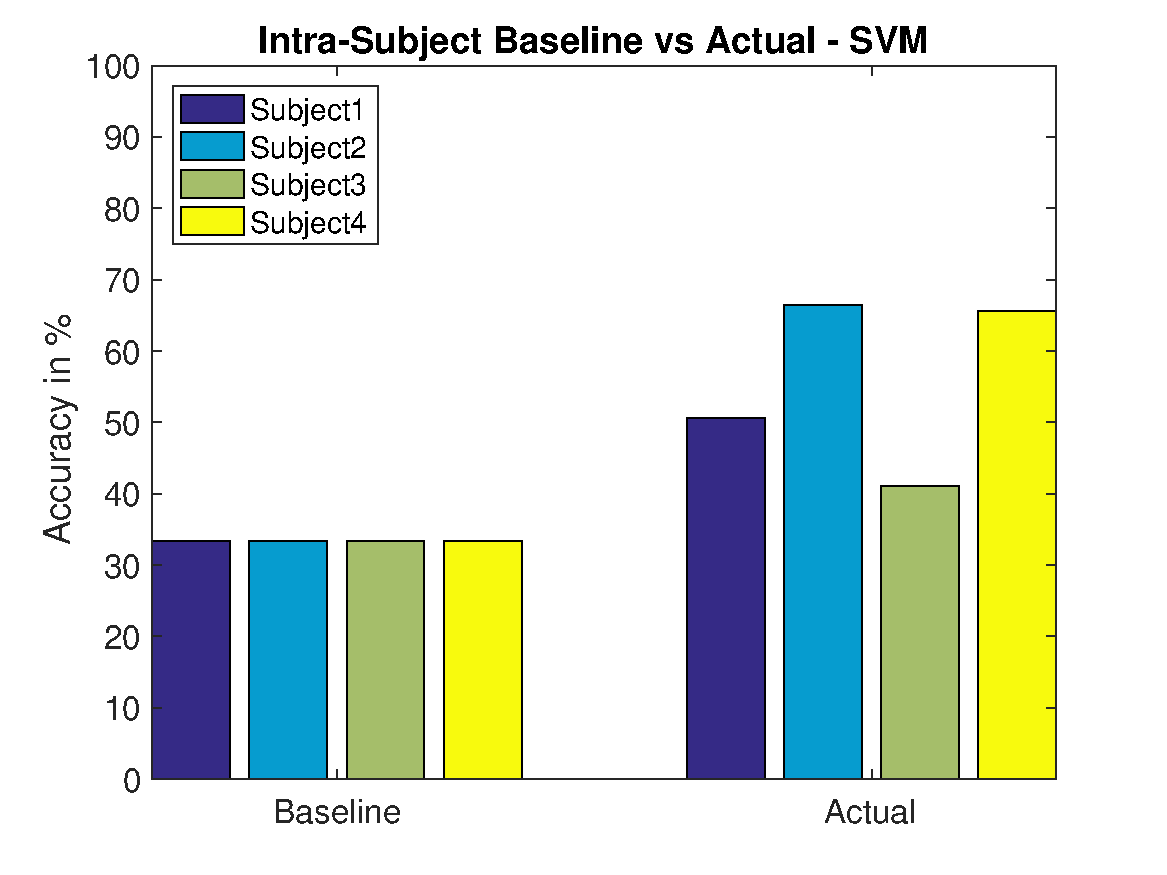
\includegraphics[width=0.90\textwidth]{Chapter-4/base_ts}
	    	\caption{Total accuracy for Intra-subject classification using the SVM Classifier}
	    	\label{fig:chap4IntraST}
    	\end{figure}

    	\begin{figure}[hbtp]
	    	\centering
	    	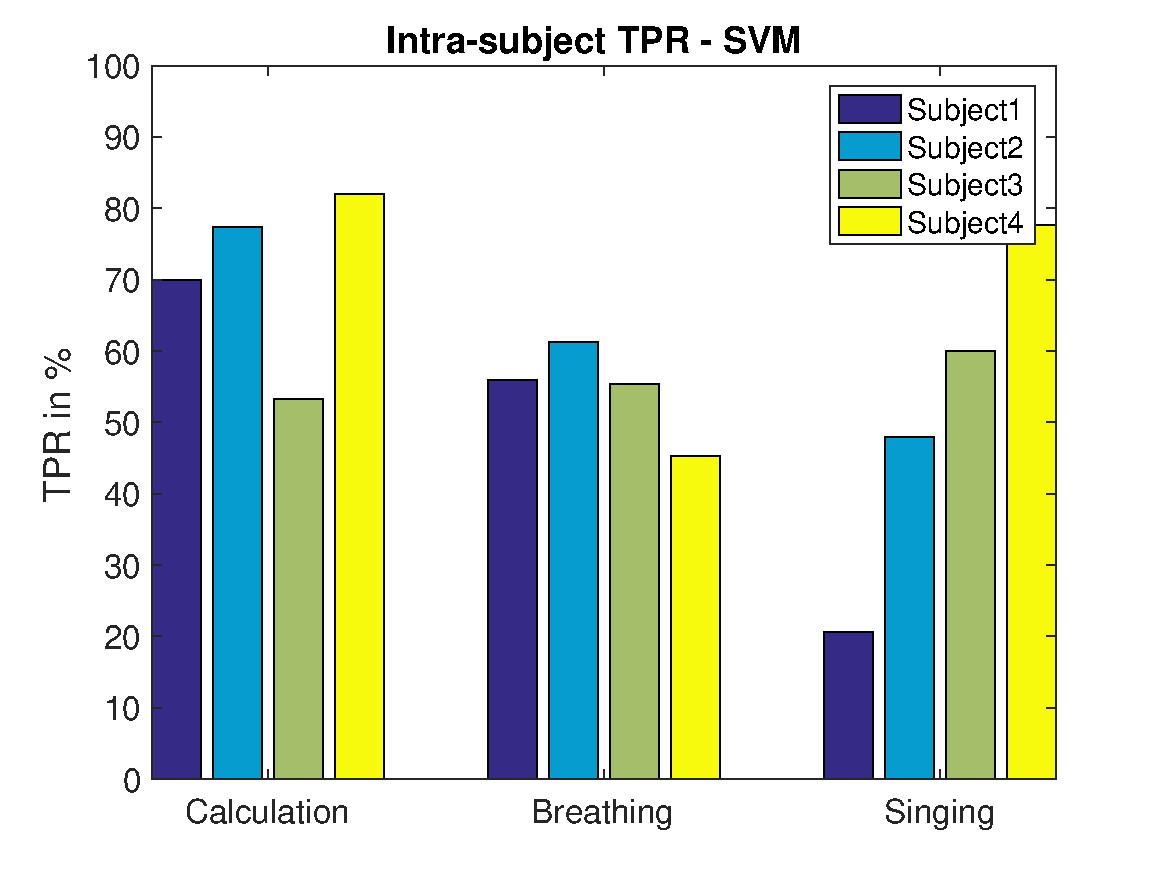
\includegraphics[width=0.9\textwidth]{Chapter-4/base_tprs}
	    	\caption{TPR for Intra-subject classification using the SVM Classifier}
	    	\label{fig:chap4IntraSTPR}
    	\end{figure}

    	\begin{figure}[hbtp]
	    	\centering
	    	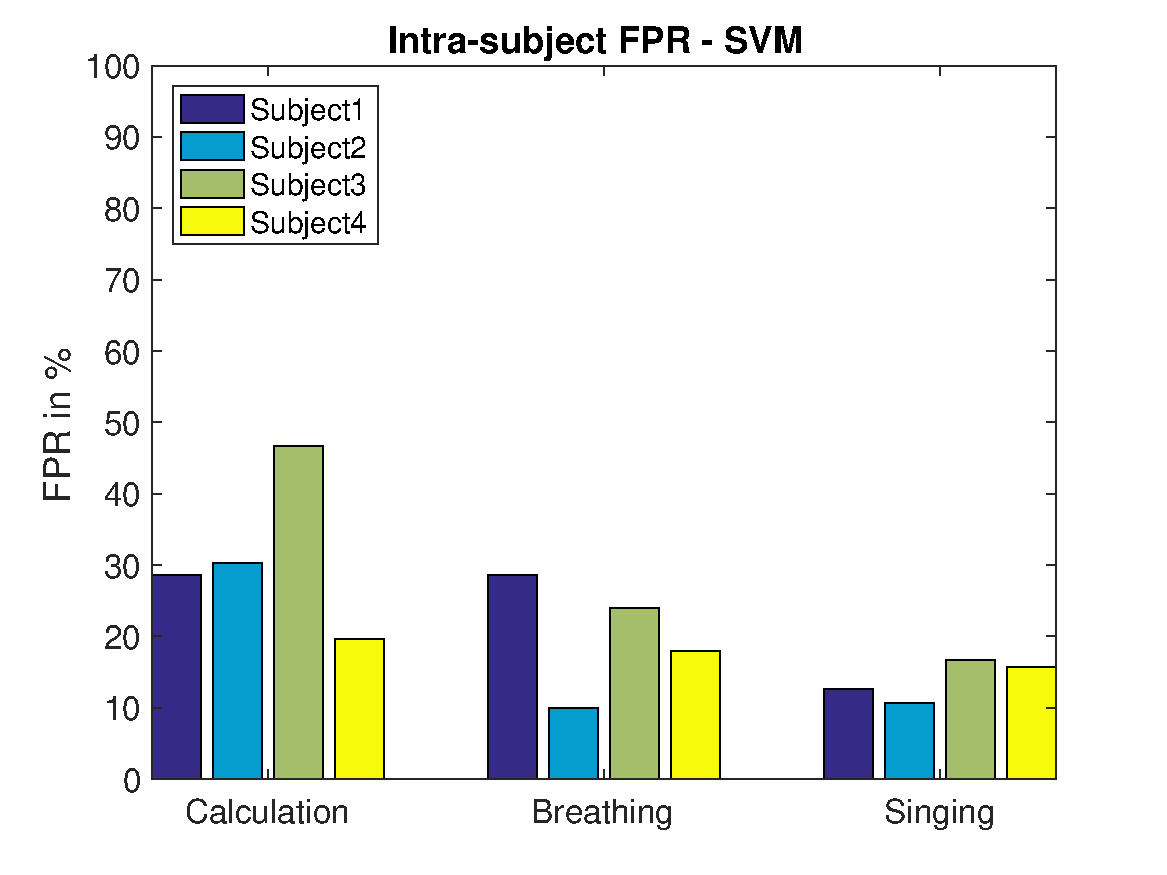
\includegraphics[width=0.90\textwidth]{Chapter-4/base_fprs}
	    	\caption{FPR for Intra-subject classification using the SVM Classifier}
	    	\label{fig:chap4IntraSFPR}
    	\end{figure}

		\begin{table}[h!]
			\centering
			\caption{Intra-subject Classification using Support Vector Machines, TPR for Calculation, Breathing and Singing Task}
			\label{SICTPR}
			\subfloat[Calculation]{
			\begin{tabular}{c c c c}
				\hline
				Sub &Min &Max &Average\\\hline
				1 &53.33 &86.67 &70.00\\
				2 &60.00 &93.33 &77.33\\
				3 &40.00 &73.33 &53.33\\
				4 &73.33 &93.33 &82.00\\
			\end{tabular}
			}\hfill
			\subfloat[Breathing]{
			\begin{tabular}{c c c c}
				\hline
				Sub &Min &Max &Average\\\hline
				1 &40.00 &73.33 &56.00\\
				2 &33.33 &73.33 &61.33\\
				3 &40.00 &73.33 &55.33\\
				4 &40.00 &66.67 &45.33\\
			\end{tabular}
			}\\
			\subfloat[Singing]{
			\begin{tabular}{c c c c}
				\hline
				Sub &Min &Max &Average\\\hline
				1 &6.67 &40.00  &20.67\\
				2 &33.33 &66.67 &48.00\\
				4 &46.67 &73.33 &60.00\\
				4 &68.67 &77.00 &77.67\\
			\end{tabular}
			}
		\end{table}

		\begin{table}[h!]
			\centering
			\caption{Intra-subject Classification using Support Vector Machines, FPR for Calculation, Breathing and Singing Task}
			\label{SICFPR}
			\subfloat[Calculation]{
			\begin{tabular}{c c c c}
				\hline
				Sub &Min &Max &Average\\\hline
				1 &20.00 &36.67 &28.67\\
				2 &23.33 &40.00 &30.33\\
				3 &36.67 &60.00 &46.67\\
				4 &10.00 &33.33 &19.67\\
			\end{tabular}
			}\hfill
			\subfloat[Breathing]{
			\begin{tabular}{c c c c}
				\hline
				Sub &Min &Max &Average\\\hline
				1 &16.67 &60.00 &28.67\\
				2 &0.00 &20.00  &10.00\\
				3 &13.33 &40.00 &24.00\\
				4 &6.67 &40.00  &18.00\\
			\end{tabular}
			}\\
			\subfloat[Singing]{
			\begin{tabular}{c c c c}
				\hline
				Sub &Min &Max &Average\\\hline
				1 &3.33 &26.67 &12.67\\
				2 &3.33 &20.00 &10.67\\
				3 &6.67 &33.33 &16.67\\
				4 &0.00 &23.33 &15.67\\
			\end{tabular}
			}
		\end{table}
		\FloatBarrier

	\subsection{Inter-Subject Classification}
    For this experiment, we collected data from four different test subjects performing three different tasks repeated five times each. As discussed in Section \ref{Chap3:Classifiers}, training and testing split was 70\% and 30\% respectively.
    \subsubsection{Mahalanobis Distance}
    Table \ref{InMD} and Figure \ref{fig:chap4InterMT} show the overall accuracy of the Mahalanobis distance classifier for inter-subject classification. Table \ref{InMDTPR} and Figure \ref{fig:chap4InterMTPR} show the TPR for different test subjects using the Mahalanobis distance classifier. Also, Table \ref{InMDFPR} and Figure \ref{fig:chap4InterMFPR} show the FPR for different test subjects using the Mahalanobis distance classifier.
		\begin{table}[h!]
			\centering
			\caption{Inter-subject Classification for 4 subjects using Mahalanobis Distance - Total Accuracy}
			\label{InMD}
			\begin{tabular}{l c c c}
				\hline
				Task &Min &Max &Average\\\hline
				Calculation &65.00 &85.00 &75.50\\
				Breathing &50.00 &65.00   &57.67\\
				Singing &55.00 &78.33     &69.00\\
			\end{tabular}
		\end{table}

		\begin{figure}[hbtp]
	    	\centering
	    	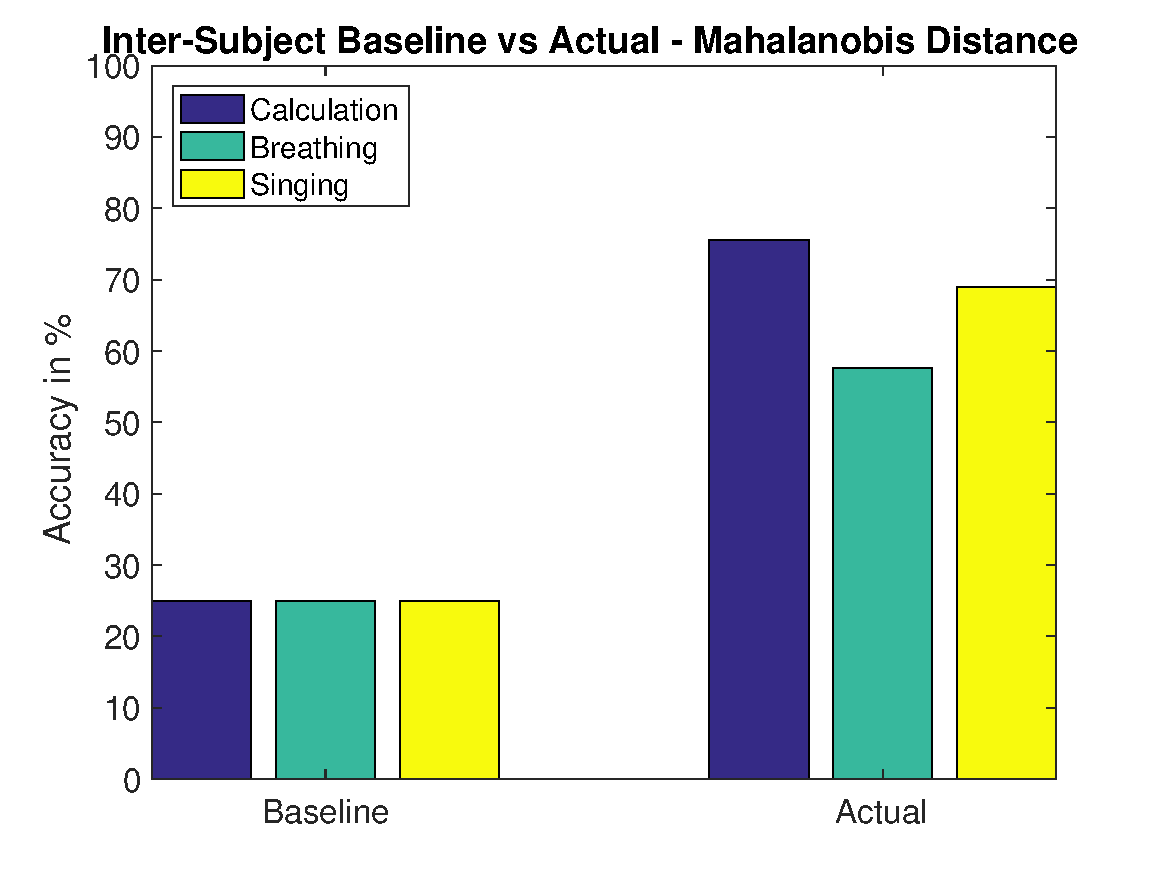
\includegraphics[width=0.90\textwidth]{Chapter-4/base_tim}
	    	\caption{Total accuracy for Inter-subject classification using the Mahalanobis Distance Classifier}
	    	\label{fig:chap4InterMT}
    	\end{figure}

    	\begin{figure}[hbtp]
	    	\centering
	    	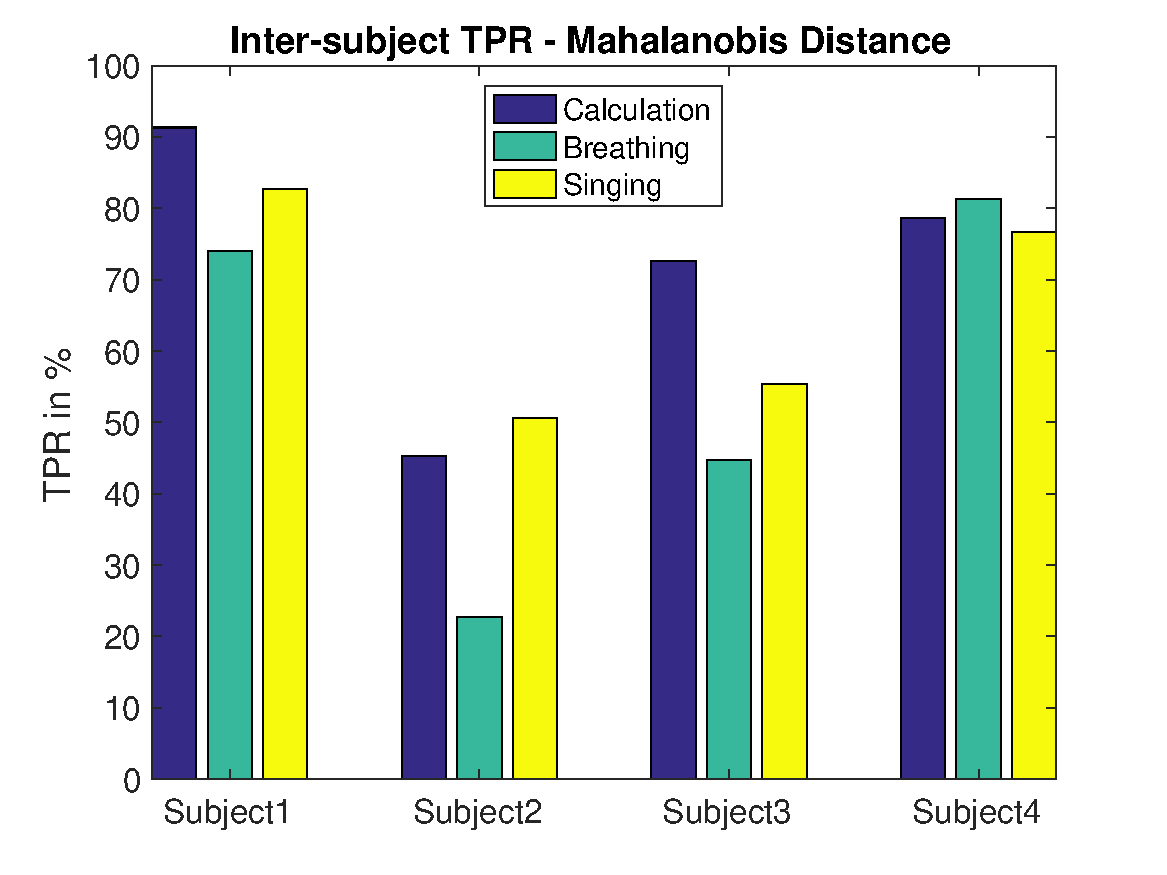
\includegraphics[width=0.90\textwidth]{Chapter-4/base_tprim}
	    	\caption{TPR for Inter-subject classification using the Mahalanobis Distance Classifier}
	    	\label{fig:chap4InterMTPR}
    	\end{figure}

    	\begin{figure}[hbtp]
	    	\centering
	    	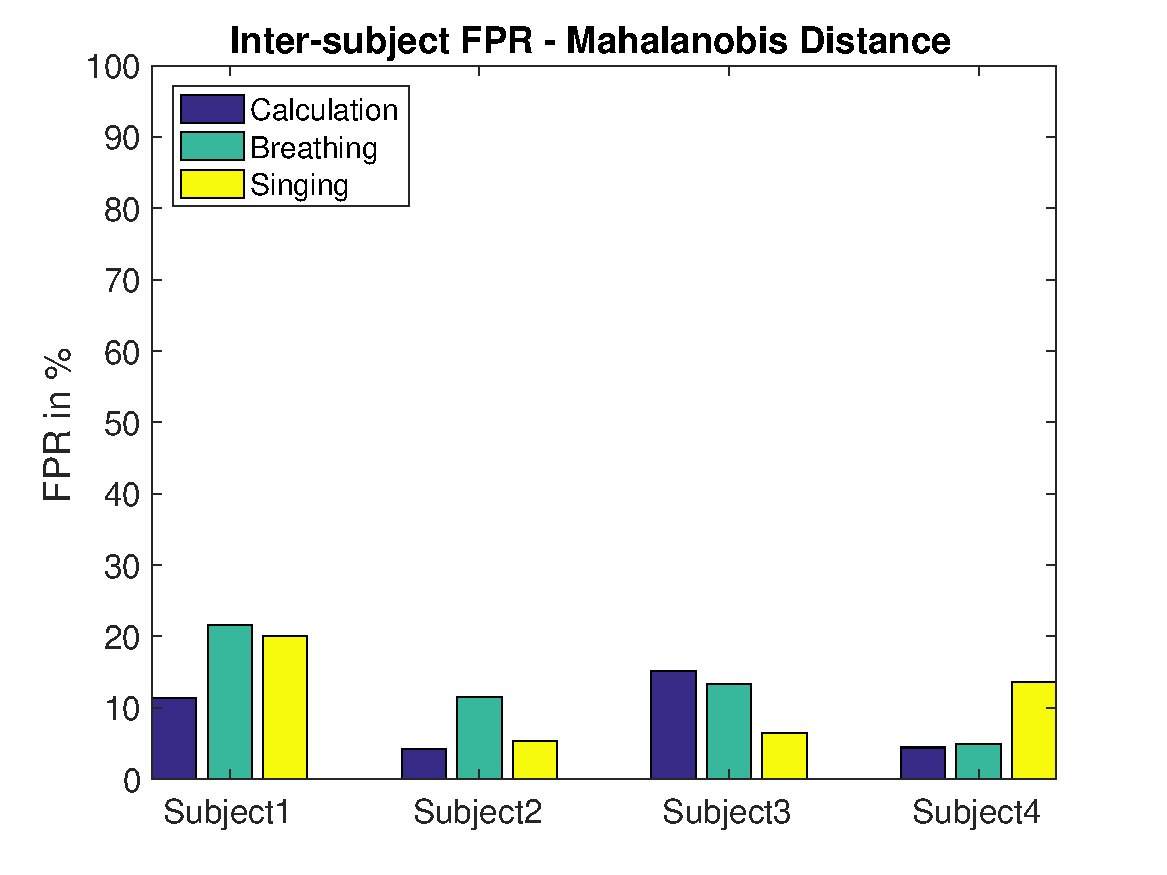
\includegraphics[width=0.90\textwidth]{Chapter-4/base_fprim}
	    	\caption{FPR for Inter-subject classification using the Mahalanobis Distance Classifier}
	    	\label{fig:chap4InterMFPR}
    	\end{figure}

		\begin{table}[h!]
			\centering
			\caption{Inter-subject Classification for 4 subjects using Mahalanobis Distance - TPR for Subject 1-4}
			\label{InMDTPR}
			\subfloat[Subject 1]{
			\begin{tabular}{l c c c}
				\hline
				Task &Min &Max &Average\\\hline
				Calculation &80.00 &100.00 &91.33\\
				Breathing &60.00 &93.33    &74.00\\
				Singing &73.33 &100.00     &82.67\\
			\end{tabular}
			}\hfill
			\subfloat[Subject 2]{
			\begin{tabular}{l c c c}
				\hline
				Task &Min &Max &Average\\\hline
				Calculation &20.00 &66.67 &45.33\\
				Breathing &6.67 &40.00    &22.67\\
				Singing &33.33 &73.33     &50.67\\
			\end{tabular}
			}\\		
			\subfloat[Subject 3]{
			\begin{tabular}{l c c c}
				\hline
				Task &Min &Max &Average\\\hline
				Calculation &46.67 &93.33 &72.67\\
				Breathing &26.67 &73.33   &44.67\\
				Singing &33.33 &73.33     &55.33\\
			\end{tabular}
			}\hfill
			\subfloat[Subject 4]{
			\begin{tabular}{l c c c}
				\hline
				Task &Min &Max &Average\\\hline
				Calculation &60.00 &86.67 &78.67\\
				Breathing &66.67 &100.00  &81.33\\
				Singing &46.67 &93.33     &76.67\\
			\end{tabular}
			}
		\end{table}

		\begin{table}[h!]
			\centering
			\caption{Inter-subject Classification for 4 subjects using Mahalanobis Distance - FPR for Subject 1-4}
			\label{InMDFPR}
			\subfloat[Subject 1]{
			\begin{tabular}{l c c c}
				\hline
				Task &Min &Max &Average\\\hline
				Calculation &2.22 &17.78 &11.33\\
				Breathing &13.33 &31.11  &21.56\\
				Singing &6.67 &35.56     &20.00\\
			\end{tabular}
			}\hfill
			\subfloat[Subject 2]{
			\begin{tabular}{l c c c}
				\hline
				Task &Min &Max &Average\\\hline
				Calculation &0.00 &8.89 &4.22\\
				Breathing &4.44 &20.00  &11.56\\
				Singing &2.22 &11.11    &5.33\\
			\end{tabular}
			}\\		
			\subfloat[Subject 3]{
			\begin{tabular}{l c c c}
				\hline
				Task &Min &Max &Average\\\hline
				Calculation &6.67 &22.22 &15.11\\
				Breathing &4.44 &28.89   &13.33\\
				Singing &2.22 &15.56     &6.44\\
			\end{tabular}
			}\hfill
			\subfloat[Subject 4]{
			\begin{tabular}{l c c c}
				\hline
				Task &Min &Max &Average\\\hline
				Calculation &2.22 &6.67 &4.44\\
				Breathing &0.00 &8.89   &4.89\\
				Singing &2.22 &28.89    &13.56\\
			\end{tabular}
			}			
		\end{table}
        
 	Inter subject classification with Mahalanobis distance demonstrate a wide variation of TPR for different test subjects. As you can see, Subject 2 and Subject 3 have lower TPR compared to Subject 3 and 4. Also, FPR for Subject 1 is higher compared to the rest of the subjects.

 	\FloatBarrier
		\subsubsection{Neural Networks}
    Table \ref{InNN} and Figure \ref{fig:chap4InterNT} show the overall accuracy of the Neural Networks classifier for inter-subject classification. Table \ref{InNNTPR} and Figure \ref{fig:chap4InterNTPR} show the TPR for different test subjects using the Neural Networks classifier. Also, Table \ref{InNNFPR} and Figure \ref{fig:chap4InterNFPR} show the FPR for different test subjects using the Neural Networks classifier.
		\begin{table}[h!]
			\centering
			\caption{Inter-subject Classification for 4 subjects using Neural Networks - Total Accuracy}
			\label{InNN}
			\begin{tabular}{l c c c}
				\hline
				Task &Min &Max &Average\\\hline
				Calculation &73.33 &85.00 &80.17\\
				Breathing &55.00 &63.33   &59.33\\
				Singing &66.67 &85.00     &73.17\\
			\end{tabular}
		\end{table}
 		
 		\begin{figure}[hbtp]
	    	\centering
	    	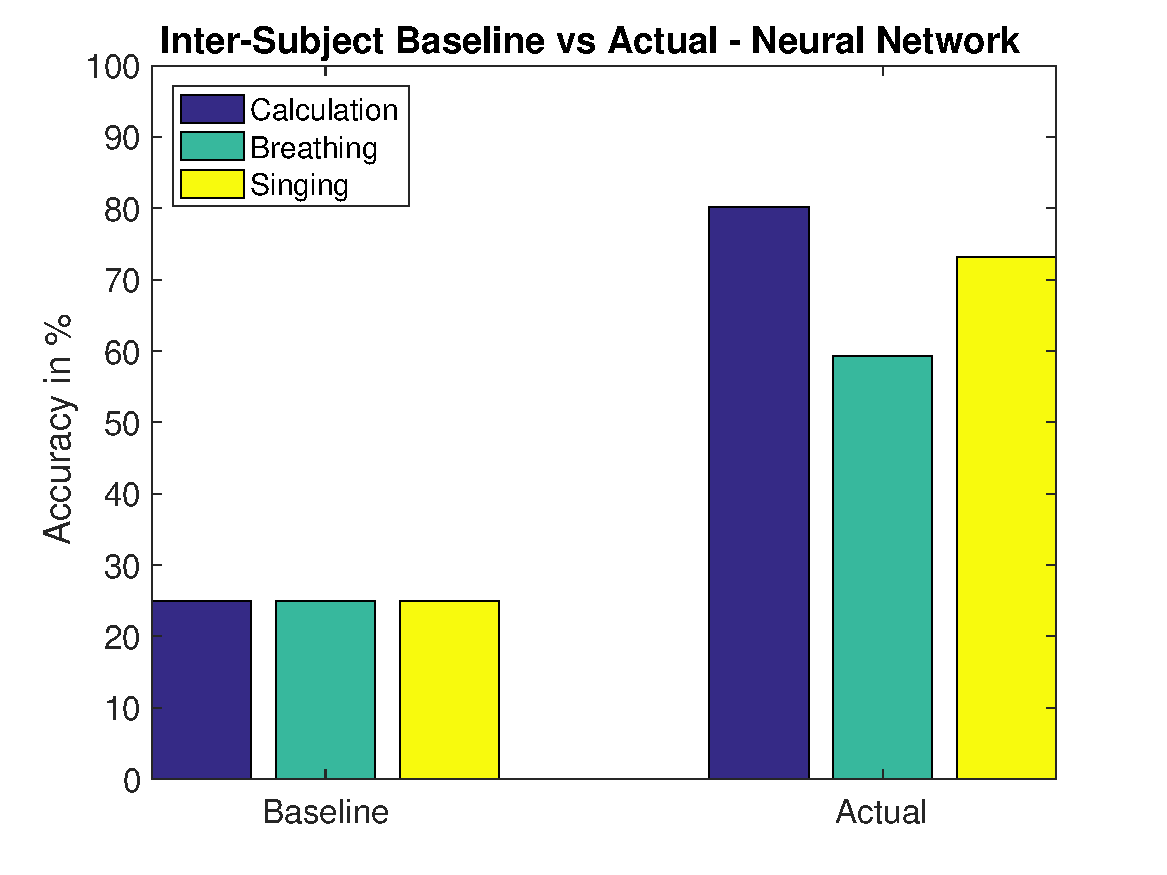
\includegraphics[width=0.90\textwidth]{Chapter-4/base_tin}
	    	\caption{Total accuracy for Inter-subject classification using Neural Networks}
	    	\label{fig:chap4InterNT}
    	\end{figure}

    	\begin{figure}[hbtp]
	    	\centering
	    	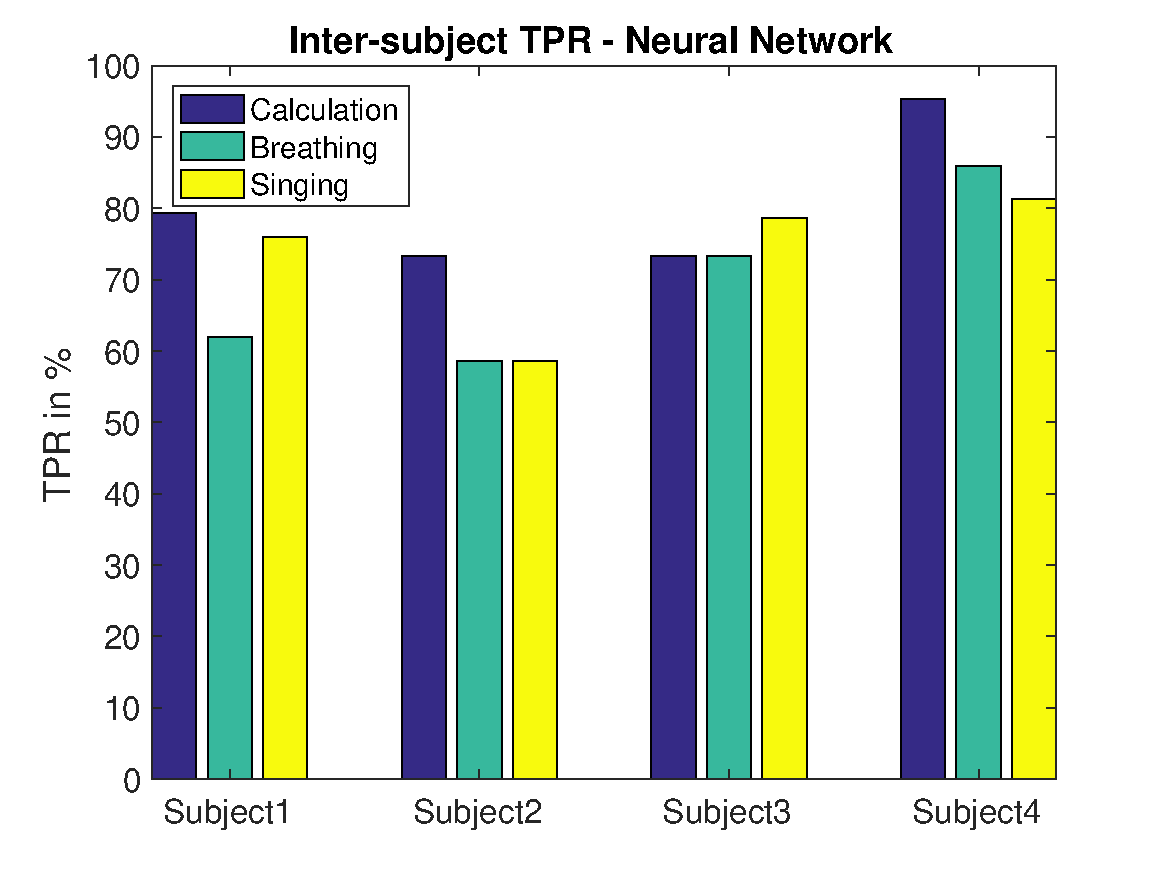
\includegraphics[width=0.90\textwidth]{Chapter-4/base_tprin}
	    	\caption{TPR for Inter-subject classification using Neural Networks}
	    	\label{fig:chap4InterNTPR}
    	\end{figure}

    	\begin{figure}[hbtp]
	    	\centering
	    	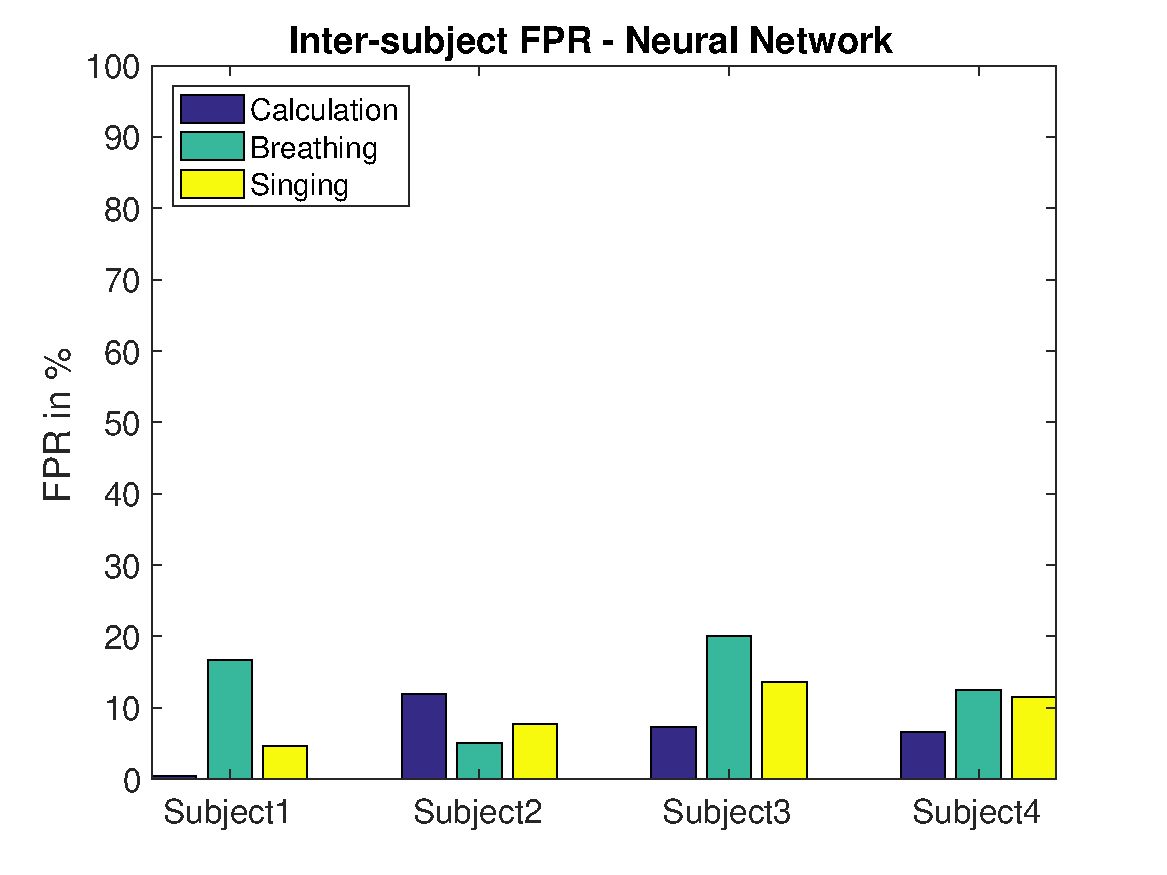
\includegraphics[width=0.90\textwidth]{Chapter-4/base_fprin}
	    	\caption{FPR for Inter-subject classification using Neural Networks}
	    	\label{fig:chap4InterNFPR}
    	\end{figure}

 		\begin{table}[h!]
			\centering
			\caption{Inter-subject Classification for 4 subjects using Neural Networks - TPR for Subject 1-4}
			\label{InNNTPR}
			\subfloat[Subject 1]{
			\begin{tabular}{l c c c}
				\hline
				Task &Min &Max &Average\\\hline
				Calculation &66.67 &86.67 &79.33\\
				Breathing &46.67 &73.33   &62.00\\
				Singing &66.67 &80.00     &76.00\\
			\end{tabular}
			}\hfill
			\subfloat[Subject 2]{
			\begin{tabular}{l c c c}
				\hline
				Task &Min &Max &Average\\\hline
				Calculation &66.67 &93.33 &73.33\\
				Breathing &26.67 &80.00   &58.67\\
				Singing &26.67 &80.00     &58.67\\
			\end{tabular}
			}\\		
			\subfloat[Subject 3]{
			\begin{tabular}{l c c c}
				\hline
				Task &Min &Max &Average\\\hline
				Calculation &60.00 &80.00 &73.33\\
				Breathing &60.00 &86.67   &73.33\\
				Singing &66.67 &93.33     &78.67\\
			\end{tabular}
			}\hfill
			\subfloat[Subject 4]{
			\begin{tabular}{l c c c}
				\hline
				Task &Min &Max &Average\\\hline
				Calculation &86.67 &100.00 &95.33\\
				Breathing &73.33 &100.00   &86.00\\
				Singing &66.67 &100.00     &81.33\\
			\end{tabular}
			}			
		\end{table}
        
		\begin{table}[h!]
			\centering
			\caption{Inter-subject Classification for 4 subjects using Neural Networks - FPR for Subject 1-4}
			\label{InNNFPR}
			\subfloat[Subject 1]{
			\begin{tabular}{l c c c}
				\hline
				Task &Min &Max &Average\\\hline
				Calculation &0.00 &2.22 &0.44\\
				Breathing &8.89 &22.22  &16.67\\
				Singing &2.22 &8.89     &4.67\\
			\end{tabular}
			}\hfill
			\subfloat[Subject 2]{
			\begin{tabular}{l c c c}
				\hline
				Task &Min &Max &Average\\\hline
				Calculation &4.44 &15.56 &12.00\\
				Breathing &0.00 &15.56   &5.11\\
				Singing &2.22 &13.33     &7.78\\
			\end{tabular}
			}\\		
			\subfloat[Subject 3]{
			\begin{tabular}{l c c c}
				\hline
				Task &Min &Max &Average\\\hline
				Calculation &0.00 &13.33 &7.33\\
				Breathing &13.33 &24.44  &20.00\\
				Singing &8.89 &17.78     &13.56\\
			\end{tabular}
			}\hfill
			\subfloat[Subject 4]{
			\begin{tabular}{l c c c}
				\hline
				Task &Min &Max &Average\\\hline
				Calculation &0.00 &11.11 &6.67\\
				Breathing &6.67 &22.22   &12.44\\
				Singing &6.67 &17.78     &11.56\\
			\end{tabular}
			}		
		\end{table}
        
        Inter-subject classification using Neural Networks show more consistency with TPR and FPR compared to Mahalanobis Distance. Also, the TPR and classification accuracy for calculation task is higher compared to breathing and song tasks.
        
        \FloatBarrier
		\subsubsection{Support Vector Machines}
    Table \ref{InSVM} and Figure \ref{fig:chap4InterST} show the overall accuracy of the SVM classifier for inter-subject classification. Table \ref{InSVMTPR} and Figure \ref{fig:chap4InterSTPR} show the TPR for different test subjects using the SVM classifier. Also, Table \ref{InSVMFPR} and Figure \ref{fig:chap4InterSFPR} show the FPR for different test subjects using the SVM classifier.        
		\begin{table}[h!]
			\centering
			\caption{Inter-subject Classification for 4 subjects using Support Vector Machines - Total Accuracy}
			\label{InSVM}
			\begin{tabular}{l c c c}
				\hline
				Task &Min &Max &Average\\\hline
				Calculation &68.33 &80.00 &76.50\\
				Breathing &50.00 &60.00   &55.17\\
				Singing &66.67 &85.00     &75.00\\
			\end{tabular}
		\end{table}

		\begin{figure}[hbtp]
	    	\centering
	    	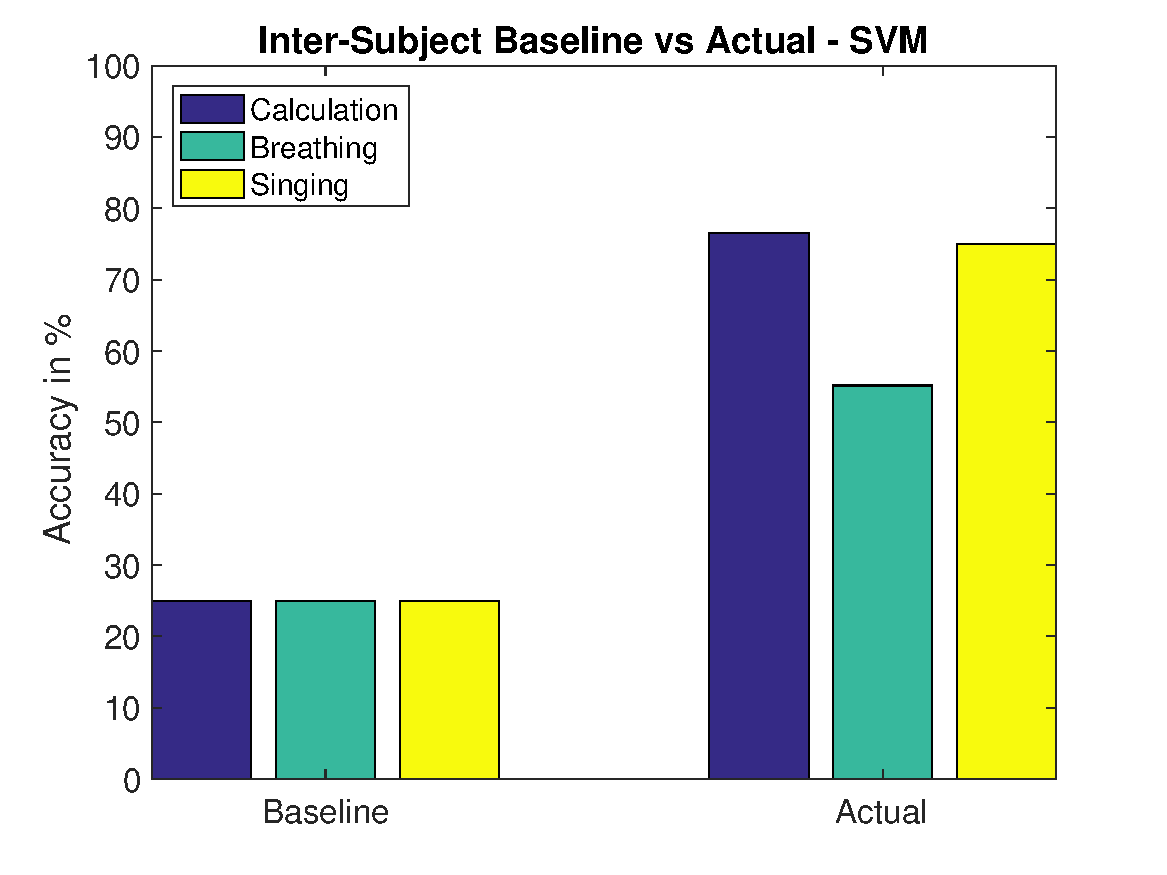
\includegraphics[width=0.90\textwidth]{Chapter-4/base_tis}
	    	\caption{Total accuracy for Inter-subject classification using Support Vector Machines}
	    	\label{fig:chap4InterST}
    	\end{figure}

    	\begin{figure}[hbtp]
	    	\centering
	    	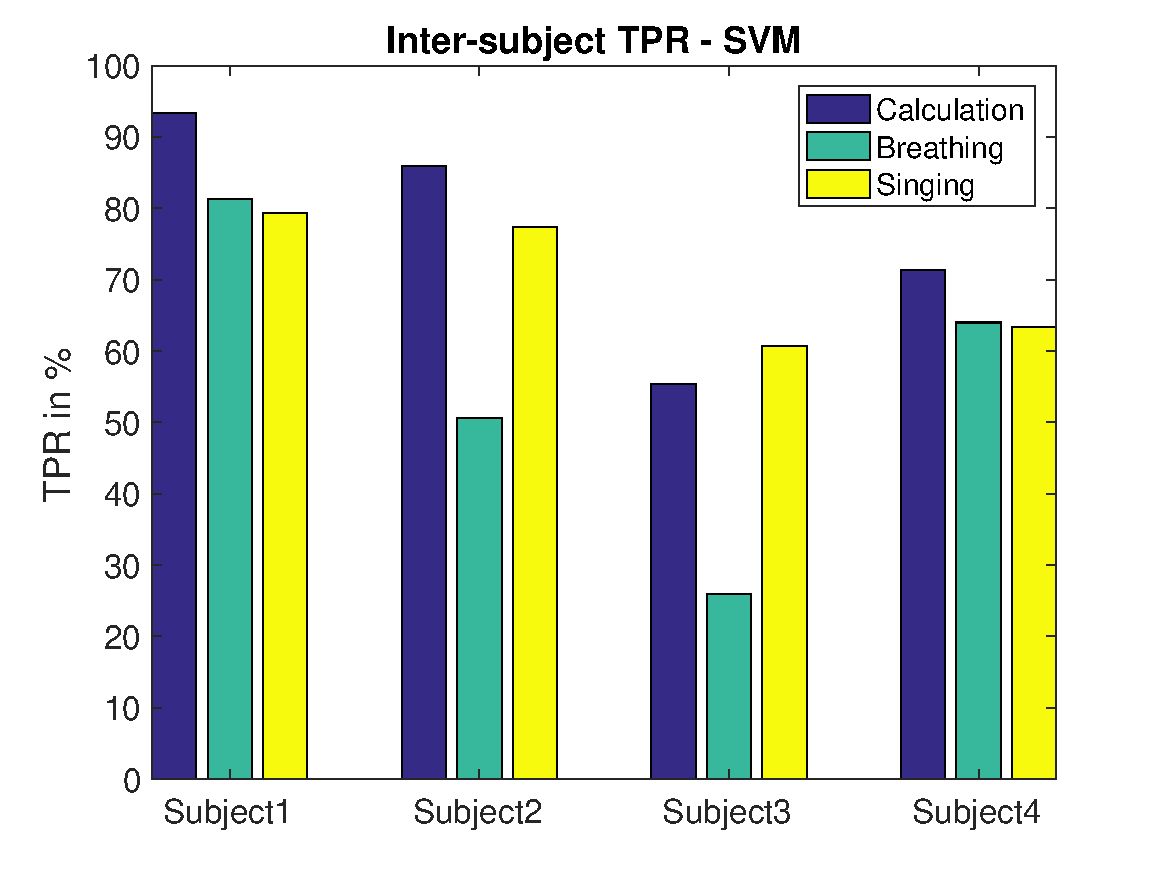
\includegraphics[width=0.90\textwidth]{Chapter-4/base_tpris}
	    	\caption{TPR for Inter-subject classification using Support Vector Machines}
	    	\label{fig:chap4InterSTPR}
    	\end{figure}

    	\begin{figure}[hbtp]
	    	\centering
	    	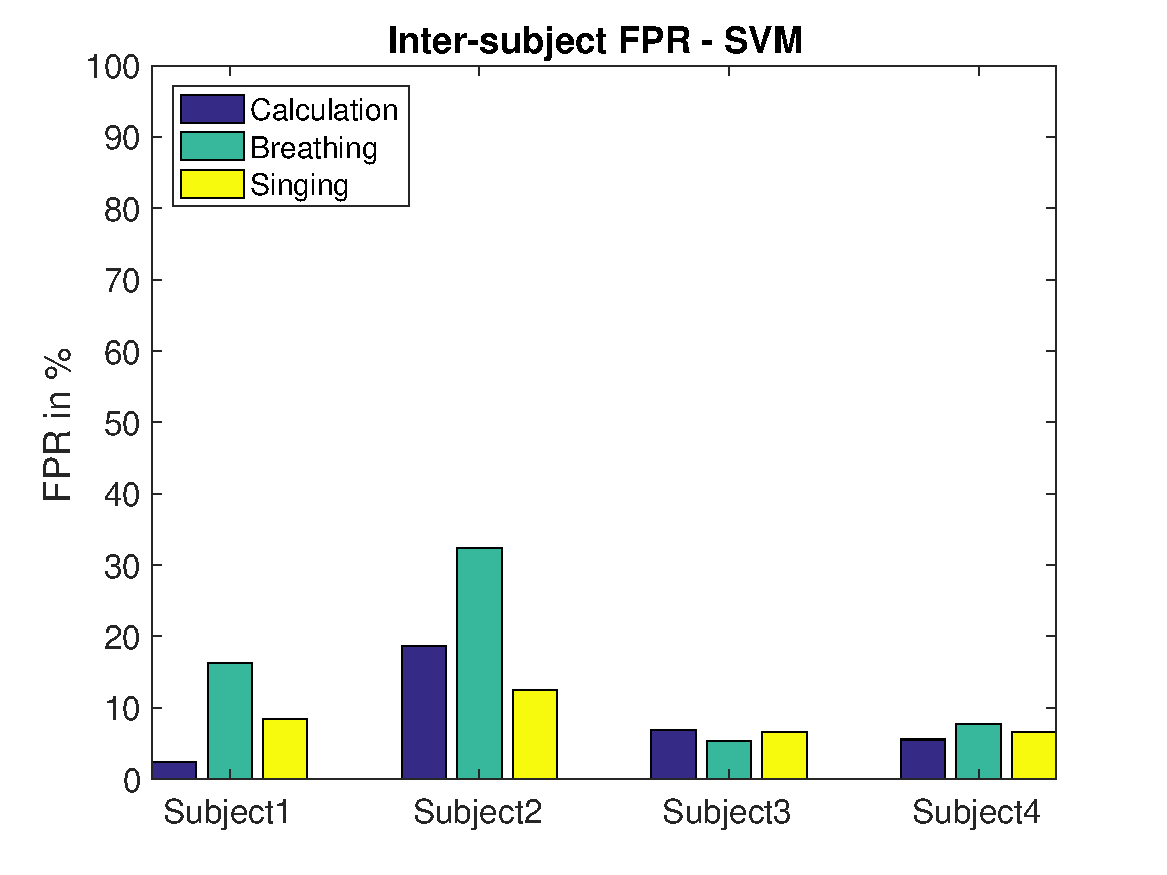
\includegraphics[width=0.90\textwidth]{Chapter-4/base_fpris}
	    	\caption{FPR for Inter-subject classification using Support Vector Machines}
	    	\label{fig:chap4InterSFPR}
    	\end{figure}

        
		\begin{table}[h!]
			\centering
			\caption{Inter-subject Classification for 4 subjects using Support Vector Machines - TPR for Subject 1}
			\label{InSVMTPR}
			\subfloat[Subject 1]{
			\begin{tabular}{l c c c}
				\hline
				Task &Min &Max &Average\\\hline
				Calculation &86.67 &100.00 &93.33\\
				Breathing &66.67 &93.33    &81.33\\
				Singing &60.00 &100.00     &79.33\\
			\end{tabular}
			}
			\subfloat[Subject 2]{
			\begin{tabular}{l c c c}
				\hline
				Task &Min &Max &Average\\\hline
				Calculation &80.00 &100.00 &86.00\\
				Breathing &20.00 &80.00    &50.67\\
				Singing &66.67 &86.67      &77.33\\
			\end{tabular}
			}\\		
			\subfloat[Subject 3]{
			\begin{tabular}{l c c c}
				\hline
				Task &Min &Max &Average\\\hline
				Calculation &40.00 &73.33 &55.33\\
				Breathing &13.33 &33.33   &26.00\\
				Singing &40.00 &73.33     &60.67\\
			\end{tabular}
			}
			\subfloat[Subject 4]{
			\begin{tabular}{l c c c}
				\hline
				Task &Min &Max &Average\\\hline
				Calculation &46.67 &93.33 &71.33\\
				Breathing &46.67 &80.00   &64.00\\
				Singing &33.33 &86.67     &63.33\\
			\end{tabular}
			}
		\end{table}
        
		\begin{table}[h!]
			\centering
			\caption{Inter-subject Classification for 4 subjects using Support Vector Machines - FPR for Subject 1}
			\label{InSVMFPR}
			\subfloat[Subject 1]{
			\begin{tabular}{l c c c}
				\hline
				Task &Min &Max &Average\\\hline
				Calculation &0.00 &6.67 &2.44\\
				Breathing &8.89 &24.44  &16.22\\
				Singing &2.22 &17.78    &8.44\\
			\end{tabular}
			}\hfill
			\subfloat[Subject 2]{
			\begin{tabular}{l c c c}
				\hline
				Task &Min &Max &Average\\\hline
				Calculation &11.11 &31.11 &18.67\\
				Breathing &24.44 &40.00   &32.44\\
				Singing &8.89 &22.22      &12.44\\
			\end{tabular}
			}\\		
			\subfloat[Subject 3]{
			\begin{tabular}{l c c c}
				\hline
				Task &Min &Max &Average\\\hline
				Calculation &2.22 &8.89 &6.89\\
				Breathing &0.00 &13.33  &5.33\\
				Singing &2.22 &11.11    &6.67\\
			\end{tabular}
			}\hfill
			\subfloat[Subject 4]{
			\begin{tabular}{l c c c}
				\hline
				Task &Min &Max &Average\\\hline
				Calculation &0.00 &8.89 &5.56\\
				Breathing &4.44 &17.78  &7.78\\
				Singing &2.22 &15.56    &6.67\\
			\end{tabular}
			}			
		\end{table}

        \FloatBarrier